\documentclass[12pt,a4paper,zihao=-4,AutoFakeBold,AutoFakeSlant]{ctexart}

% ---------------------
% 中文与字体设置（ctex 已包含 xeCJK 与 fontspec）
% ---------------------
\usepackage{setspace}  % 行间距

% ---------------------
% 数学公式
% ---------------------
\usepackage{amsmath, amsthm, amssymb, amsfonts, mathrsfs, mathtools}

% ---------------------
% 图形与表格
% ---------------------
\usepackage{graphicx, caption, subcaption, float}
\usepackage{array, tabularx, multirow}

% ---------------------
% 页面与排版
% ---------------------
\usepackage{geometry, fancyhdr}
\usepackage{framed, mdframed}
\usepackage{enumitem} % 更灵活控制列表格式
\usepackage{tocloft, booktabs}
% ---------------------
% 算法与代码
% ---------------------
\usepackage[boxed,ruled,lined,linesnumbered]{algorithm2e}
\usepackage{algorithmic}
\usepackage{listings, lstautogobble}
\usepackage{minted}  % 需要 XeLaTeX 或 LuaLaTeX 支持

% ---------------------
% 参考文献
% ---------------------
\usepackage[backend=biber, style=numeric, sorting=none]{biblatex}
\addbibresource{ref.bib}

% ---------------------
% 其他工具包
% ---------------------
\usepackage{appendix}
\usepackage{tablefootnote}
\usepackage[colorlinks, linkcolor=black, anchorcolor=black, citecolor=black]{hyperref}
\usepackage[symbol]{footmisc}
\usepackage{cleveref}
\usepackage{color, xcolor}
\usepackage{xlop}

% 页面格式
\geometry{left=3cm,right=3cm,top=2.5cm,bottom=2.5cm}

% 目录和正文的页眉与页脚
\fancypagestyle{plain}
 {\fancyhf{}
  \fancyfoot[C]{\zihao{-5}\thepage}
  \renewcommand\headrulewidth{0pt}
  \renewcommand\footrulewidth{0pt}}
\fancypagestyle{body}
 {\fancyhf{}
  \fancyfoot[C]{\zihao{-5}\thepage}
  \fancyhead{\centering\zihao{-5}机器学习课程论文}
  \renewcommand\headrulewidth{0.6pt}
  \renewcommand\footrulewidth{0pt}}

% 字体设置
\setmainfont{Times New Roman}

% 修改 \supercite 格式，加上带中括号的右上标
\makeatletter
\DeclareCiteCommand{\supercite}[\mkbibsuperscript]
  {\let\multicitedelim=\supercitedelim
   \usebibmacro{prenote}}
  {\usebibmacro{citeindex}%
   \usebibmacro{cite}}
  {\multicitedelim}
  {\usebibmacro{postnote}}
\renewcommand{\mkbibsuperscript}[1]{\textsuperscript{\normalfont[#1]}}  % 添加 \normalfont 防止字体混乱
\makeatother

\ctexset{
  section={
    format+=\heiti\zihao{3}\bfseries,
    beforeskip=0.8\baselineskip,
    afterskip=0.5\baselineskip,
  },
  subsection={
    format=\heiti\zihao{4}\bfseries,
    beforeskip=0.5\baselineskip,
    afterskip=0.5\baselineskip,
  },
  subsubsection={
    format=\heiti\zihao{-4}\bfseries,
    beforeskip=0.5\baselineskip,
    afterskip=0.5\baselineskip,
  },
  autoindent=true,
  contentsname={\hfill\textbf{\heiti\zihao{-2}目\qquad 录}\hfill},
  bibname={\hfill\heiti\zihao{-2}{参考文献}\hfill},
  appendixname={\hfill\textbf{\heiti\zihao{-2}附\qquad 录}\hfill},
}

% 设置片和表格编号的格式
\renewcommand{\thefigure}{\arabic{section}.\arabic{figure}}
\renewcommand{\thetable}{\arabic{section}-\arabic{table}}
\DeclareCaptionLabelSeparator{quad}{\quad}
\captionsetup{labelsep=quad, font=small, labelfont=bf, skip=6pt}
\captionsetup[sub]{labelsep=space, font=small, labelfont=rm}

\lstset{
    language=Python,
    basicstyle=\fontspec{Noto Sans Mono}\scriptsize,  % 设置代码字体
    keywordstyle=\color{blue},              % 设置关键字颜色
    commentstyle=\color{purple},      % 设置注释颜色
    stringstyle=\color{black},     % 设置字符串颜色
    backgroundcolor=\color{white},          % 设置背景颜色为白色
    frame=single,                           % 绘制单线框架
    xleftmargin=0.5em,                      % 设置左边距
    xrightmargin=0em,                       % 设置右边距
    rulecolor=\color{darkgray},             % 设置框架线颜色为深灰
    stepnumber=1,                           % 每行都显示行号
    numbers=left,                           % 将行号显示在左侧
    numberstyle=\tiny\color{black},         % 设置行号的格式
    numbersep=5pt,                          % 设置行号和代码之间的间距
    breaklines=true,                        % 允许自动换行
    breakatwhitespace=true,                 % 仅在空格处换行
    columns=flexible,                       % 设置列宽度自动调整
    escapeinside={*@}{@*},                  % 允许使用特定符号插入LaTeX命令
    showstringspaces=false,                 % 不显示字符串中的空格
    showspaces=false,                       % 不显示空格
    showtabs=false,                         % 不显示制表符
    tabsize=2,                              % 设置制表符宽度为2个空格
    extendedchars=true,                     % 允许使用扩展字符
    alsoletter={.},                         % 将句点视为字母
    sensitive=true,
    keywords={
        True, False, None, and, as, assert, async, await, break, class, continue, def, del,
        elif, else, except, finally, for, from, global, if, import, in, is, lambda, nonlocal,
        not, or, pass, raise, return, try, while, with, yield, list, dict, set, tuple, range, zip
    },
    alsoother={=, +, -, *, /, //, **, ==, !=, <, <=, >, >=, +=, -=, *=, /=, **=, //=, \%},
    linewidth=\textwidth,                   % 设置行宽为文本宽度
    breakautoindent=true,                   % 保持缩进
    keepspaces=true,                        % 保持空格
    moredelim=[is][\bfseries\color{green}]{~}{~},  % 设置特殊字符的颜色
}

\begin{document}

\pagestyle{empty}

\newpage\begin{figure}[t]
  \centering
  
\includegraphics[width=0.8\linewidth]{pic/cover.jpg}
\end{figure}

\begin{center}
  \fontsize{66pt}{0}
  \heiti
  \punctstyle{banjiao}
  \scalebox{0.68}[1.0]{课\qquad 程\qquad 论\qquad 文}
\end{center}

\begin{center}
  \heiti
  \zihao{-2}
  论文题目：基于视觉Transformer的印刷体与手写体数学表达式识别与LaTeX转换研究
\end{center}

\vspace{\fill}

\begin{table}[h]
  \renewcommand\arraystretch{2}
  \centering
  \songti
  \zihao{4}
  \begin{tabularx}{20em}{l>{\centering\arraybackslash}X}
    \textbf{\kaishu 学\qquad 院} & 数学与统计学院 \\
    \cline{2-2}
    \textbf{\kaishu 班\qquad 级} & 2021 级 统计学2 班\\
    \cline{2-2}
    \textbf{\kaishu 姓\qquad 名} & 李袖印 \\
    \cline{2-2}
    \textbf{\kaishu 学\qquad 号} & 202100820077 \\
    \cline{2-2}
  \end{tabularx}
\end{table}

\vspace{\fill}

\begin{table}[h]
  \renewcommand\arraystretch{2}
  \kaishu
  \centering
  \begin{tabular}{clclcl}
    2025 & 年 & 6 & 月 & 30 & 日 \\
  \end{tabular}
\end{table}


\begin{sloppypar}
  \newpage\section*{\heiti\zihao{-2}摘\qquad 要}

数学表达式识别与LaTeX生成是计算机视觉与自然语言处理交叉领域的重要研究课题，在文档数字化、教育辅助和学术研究等领域具有广泛应用前景。
传统方法多依赖卷积神经网络处理数学表达式图像，受限于局部感受野，难以建模数学符号间的长程结构依赖；而手写体表达式因笔迹风格差异大、结构层次复杂，识别难度进一步加剧。
为此，本文基于 PyTorch 实现了一种以 Vision Transformer（ViT）为编码器、标准 Transformer 为解码器的端到端模型框架，实现数学表达式图像的结构化识别及 LaTeX 序列生成，并在印刷体与手写体两类数据集上系统评估其性能。

模型方面，ViT 编码器将输入图像划分为固定尺寸的图像块，通过多层预归一化 Transformer 块的自注意力机制建模图像块间的全局依赖；解码器结合因果自注意力与交叉注意力机制，分别建模目标序列内部的上下文依赖以及与图像编码表示之间的对齐关系，输出层叠加基于训练语料词频的对数先验偏置。
训练方面，采用掩蔽交叉熵损失忽略填充位置、AdamW 优化器配合 Transformer 预热—衰减学习率调度与全局范数梯度裁剪、固定随机种子的验证集划分以及早停机制；推理阶段实现贪婪解码与带 GNMT 长度惩罚的束搜索解码。

实验在印刷体数据集 \texttt{im2latex-100k} 与手写体数据集 \texttt{MathWriting-human} 上以完全相同的架构与训练配方进行。
在印刷体测试集上，模型取得 $90.14\%$ 的词元级准确率，自回归生成的 BLEU-4 分数为 $0.6767$（贪婪解码）与 $0.7012$（束搜索），以 $7.73$M 的轻量参数规模与 $50\times200$ 的低分辨率输入验证了纯 Transformer 架构在该任务上的有效性。
训练稳定性分析提供了梯度裁剪必要性的直接实验证据：在大批量配合预热调度的设定下，无裁剪训练曾在学习率峰值附近发散并坍缩为退化解，引入裁剪后训练全程平稳收敛。

手写体对比实验则定量揭示了直接迁移印刷体配方的局限：测试集词元级准确率降至 $56.63\%$，BLEU-4 为 $0.0833$，且束搜索不再带来增益。
通过对验证—测试性能鸿沟、训练曲线分化与输入几何失真的分析，本文将该性能差距分解为书写者分布偏移、训练样本量不足与宽高比失真三个可分别施治的因素，并据此提出全量数据训练、数据增强与保宽高比预处理等改进方向。

研究结果表明，基于 Vision Transformer 的端到端模型在印刷体数学表达式识别任务上具有良好的性能表现；针对手写场景的对比实验在严格控制变量的前提下刻画了跨书写者泛化的核心挑战，为后续手写数学表达式识别研究提供了可复现的基线方法与明确的改进路径。

\vspace{0.5cm}
\noindent\textbf{关键词：}手写数学表达式识别；LaTeX 转换；Vision Transformer；注意力机制；深度学习；图像识别

\end{sloppypar}

% \begin{sloppypar}
%   \newpage\section*{\zihao{-2}Abstract}

Mathematical expression recognition and LaTeX generation is an important research topic at the intersection of computer vision and natural language processing, with broad application prospects in document digitization, educational assistance, and academic research.
Traditional methods primarily rely on convolutional neural networks, whose limited receptive fields make it difficult to model long-range structural dependencies between mathematical symbols; handwritten expressions, with their large stylistic variation and complex hierarchical structures, are even more challenging.
This study implements, in PyTorch, an end-to-end framework with a Vision Transformer (ViT) encoder and a standard Transformer decoder for structural recognition of mathematical expression images and LaTeX sequence generation, and systematically evaluates it on both printed and handwritten datasets.

On the model side, the ViT encoder splits the input image into fixed-size patches and models global dependencies among them through stacked pre-norm Transformer blocks; the decoder combines causal self-attention and cross-attention to model intra-sequence context and image--text alignment respectively, with a log-frequency prior bias added to the output layer.
On the training side, the framework employs a masked cross-entropy loss that ignores padding positions, the AdamW optimizer with the warmup--decay learning rate schedule of the original Transformer and global-norm gradient clipping, a seeded random validation split, and early stopping; at inference time both greedy decoding and beam search with the GNMT length penalty are implemented.

Experiments are conducted on the printed dataset \texttt{im2latex-100k} and the handwritten dataset \texttt{MathWriting-human} with an identical architecture and training recipe.
On the printed test set, the model achieves $90.14\%$ token-level accuracy and autoregressive BLEU-4 scores of $0.6767$ (greedy) and $0.7012$ (beam search), validating the effectiveness of a pure Transformer architecture with only $7.73$M parameters and low-resolution $50\times200$ inputs.
The training stability analysis provides direct experimental evidence for the necessity of gradient clipping: under large-batch training with warmup scheduling, an unclipped run diverged near the peak learning rate and collapsed to a degenerate solution, whereas clipping kept training stable throughout.

The handwritten comparison experiment quantitatively reveals the limitations of directly transferring the printed-formula recipe: token-level accuracy drops to $56.63\%$, BLEU-4 to $0.0833$, and beam search no longer yields gains.
By analyzing the validation--test performance gap, the divergence of training curves, and input geometric distortion, this study decomposes the performance gap into three separately addressable factors --- writer distribution shift, insufficient training samples, and aspect-ratio distortion --- and accordingly proposes full-data training, data augmentation, and aspect-preserving preprocessing as improvement directions.

The results show that the ViT-based end-to-end model performs well on printed mathematical expression recognition; the strictly controlled handwritten comparison characterizes the core challenge of cross-writer generalization, providing a reproducible baseline method and a clear improvement path for subsequent research on handwritten mathematical expression recognition.

\vspace{0.5cm}
\noindent\textbf{Keywords:} Handwritten Mathematical Expression Recognition; LaTeX Conversion; Vision Transformer; Attention Mechanism; Deep Learning; Image Recognition

% \end{sloppypar}

\clearpage
\setcounter{page}{1}
\pagenumbering{Roman}
\pagestyle{plain}

\newpage
\tableofcontents

\clearpage
\setcounter{page}{1}
\pagenumbering{arabic}
\pagestyle{body}

\begin{sloppypar}
  \newpage\section{绪论}

\subsection{选题背景与研究意义}

数学表达式是科学、工程与教育领域知识表达的基本载体。然而，纸质文档、手写笔记与扫描图像中的公式往往以非结构化的图像形式存在，难以被检索、编辑与再利用。将公式图像自动转换为 LaTeX 等结构化标记语言，是文档数字化、学术文献挖掘、智能教育以及面向视障人群的无障碍辅助等应用的关键环节，具有重要的现实意义。

与一般的光学字符识别（OCR）不同，数学表达式识别（Mathematical Expression Recognition, MER）不仅要识别单个符号，更需还原符号之间的二维空间结构——上下标的层级、分式的横线、根式的辖域、矩阵与行列式的排布，以及求和、积分的上下限等。这类“结构化识别”要求模型同时具备视觉感知与语言建模能力，难度显著高于一维文本识别。其中，印刷体公式排版规范、风格统一，相对易于处理；而手写体公式因书写者风格差异大、连笔与潦草普遍、采集图像几何比例多变，识别难度进一步加剧，至今仍是公认的挑战性问题。

本文的研究任务是：给定一张数学表达式图像，端到端地生成与之对应的 LaTeX 词元序列；并在印刷体与手写体两类场景下系统地考察同一方法的性能与可迁移性。

\subsection{国内外研究现状}

早期的数学表达式识别多采用“符号分割—结构分析”的两阶段范式：先切分出单个符号，再借助二维文法或投影规则恢复其空间关系。此类方法依赖大量手工规则，对噪声、粘连与书写风格变化的鲁棒性较差，且分割误差会沿流水线累积。

随着深度学习的发展，研究者将该任务重新表述为“图像到标记”（image-to-markup）的序列生成问题。Deng 等\supercite{dengImagetomarkupGenerationCoarsetofine2017} 提出以卷积网络编码图像、循环网络结合由粗到细注意力解码的端到端框架，并整理了大规模印刷体基准 \texttt{im2latex-100k}\supercite{kanervisto_2016_56198}，奠定了该范式的基础。然而，卷积网络受限于局部感受野，难以充分建模公式中远距离符号之间的结构依赖。

Transformer\supercite{vaswaniAttentionAllYou2017} 凭借自注意力机制对全局依赖的高效建模，迅速成为序列建模的主流架构。在手写数学表达式识别方向，Zhao 等\supercite{zhaoHandwrittenMathematicalExpression2021} 提出双向训练的 Transformer 解码器（BTTR），Ung 等\supercite{ungTransformerbasedMathLanguage2021} 引入基于 Transformer 的数学语言模型，近期的 TAMER\supercite{zhuTAMERTreeawareTransformer2024} 与 PosFormer\supercite{guanPosFormerRecognizingComplex2024} 进一步将公式的树形/位置结构先验融入解码，Zhou 等\supercite{zhouEndtoendFormulaRecognition2022} 亦探索了融合注意力机制的端到端识别方法。在视觉编码方面，Dosovitskiy 等\supercite{dosovitskiyImageWorth16x162021} 提出的 Vision Transformer（ViT）证明了纯 Transformer 直接处理图像块序列的可行性，为以全局自注意力替代卷积主干提供了依据；Sundararaj 等\supercite{sundararajAutomatedLaTeXCode2024} 据此尝试以 ViT 编码手写公式并生成 LaTeX 代码，与本文的技术路线最为接近。在数据资源方面，除印刷体的 \texttt{im2latex-100k} 外，Gervais 等\supercite{gervaisMathWritingDatasetHandwritten2025} 发布的 \texttt{MathWriting} 提供了大规模真实手写样本，为手写场景的评测奠定了基础。

综观已有工作，性能领先的方法往往依赖较高分辨率的输入、专门设计的结构化解码器（如树形解码、由粗到细注意力）或较大的模型容量。相比之下，“纯 Transformer 架构（ViT 编码器 + 标准 Transformer 解码器）在低分辨率、轻量参数规模下的有效性边界”，以及“同一套架构与训练配方在印刷体与手写体之间的可迁移性”，仍缺乏系统、可控的定量刻画。这正是本文试图回答的问题。

\subsection{主要研究内容与组织架构}

围绕上述问题，本文的主要工作与贡献如下：

\begin{enumerate}[label={（\arabic*）}, leftmargin=2em, labelsep=0.5em, itemsep=0pt]
    \item 构建了一个以 Vision Transformer 为编码器、标准 Transformer 为解码器的端到端图像到 LaTeX 模型。该模型仅含约 $7.73$M 参数、接受 $50\times200$ 的低分辨率灰度输入，采用掩蔽交叉熵损失、AdamW 优化器配合 Transformer 预热—衰减学习率调度，并在输出层引入基于训练语料词频的对数先验偏置；推理阶段提供贪婪解码与带 GNMT 长度惩罚的束搜索。
    \item 以\textbf{完全相同}的架构与训练配方，在印刷体（\texttt{im2latex-100k}）与手写体（\texttt{MathWriting-human}）两类数据集上开展严格控制变量的对比实验，定量刻画了跨书写者泛化这一手写识别的核心难题，并将印刷体到手写体的性能差距系统地分解为书写者分布偏移、训练样本量不足导致的过拟合、以及输入宽高比失真三个模型与数据层面的成因，外加 BLEU 指标对短序列的放大效应这一测量层面的因素。
    \item 总结了若干可复现的工程经验：其一，在大批量、强预热的设定下，全局范数梯度裁剪并非可选项，而是保证训练可靠收敛的必要组件（本文给出了无裁剪训练在学习率峰值附近发散并坍缩为退化解的直接证据）；其二，教师强制下的逐词元准确率会系统性高估模型的实际生成能力，因而本文以自回归 BLEU-4 作为衡量真实推理性能的主要指标。
\end{enumerate}

本文其余部分组织如下：“Vision Transformer 基本原理”一章介绍注意力机制与 ViT 的核心原理；“训练原理”一章阐述评价指标、损失函数、优化器与学习率调度以及正则化策略；“模型构建”一章详述数据预处理、编码器与解码器的具体设计以及训练与推理流程；“结果与评价”一章给出实验设置、主要结果、解码策略与手写场景的对比实验，并展开误差分析、局限性讨论与改进展望。

  \newpage\section{Vision Transformer基本原理}
\subsection{经典Transformer}
Transformer 模型最初由 Google Brain 团队提出，其核心创新在于引入自注意力机制（Self-Attention Mechanism），有效建模序列中各位置之间的长距离依赖关系。相较于传统循环神经网络（RNN），该机制不仅提高了特征提取能力，还显著增强了模型的并行计算能力，从而提升了训练效率与表现效果。

Transformer 最初被广泛应用于自然语言处理领域，尤其在机器翻译任务中取得了突破性成果。然而，得益于其强大的表示能力与高度的架构灵活性，Transformer 很快被扩展至计算机视觉等多个领域。本文将首先简要回顾经典的 Transformer 模型架构及其原理\supercite{vaswaniAttentionAllYou2017}。
\subsubsection{注意力机制}
在注意力机制的背景下，自主性提示被称为查询($\boldsymbol{q} \in \mathbb{R}^{q}$)，非自主性提示被称为键($\boldsymbol{k}\in \mathbb{R}^{k}$)。
注意力汇聚将给定的查询与键进行匹配，最终根据所得的注意力权重得出最匹配的值。
\begin{figure}[H]
  \centering
  \begin{subfigure}[b]{0.48\textwidth}
    \centering
    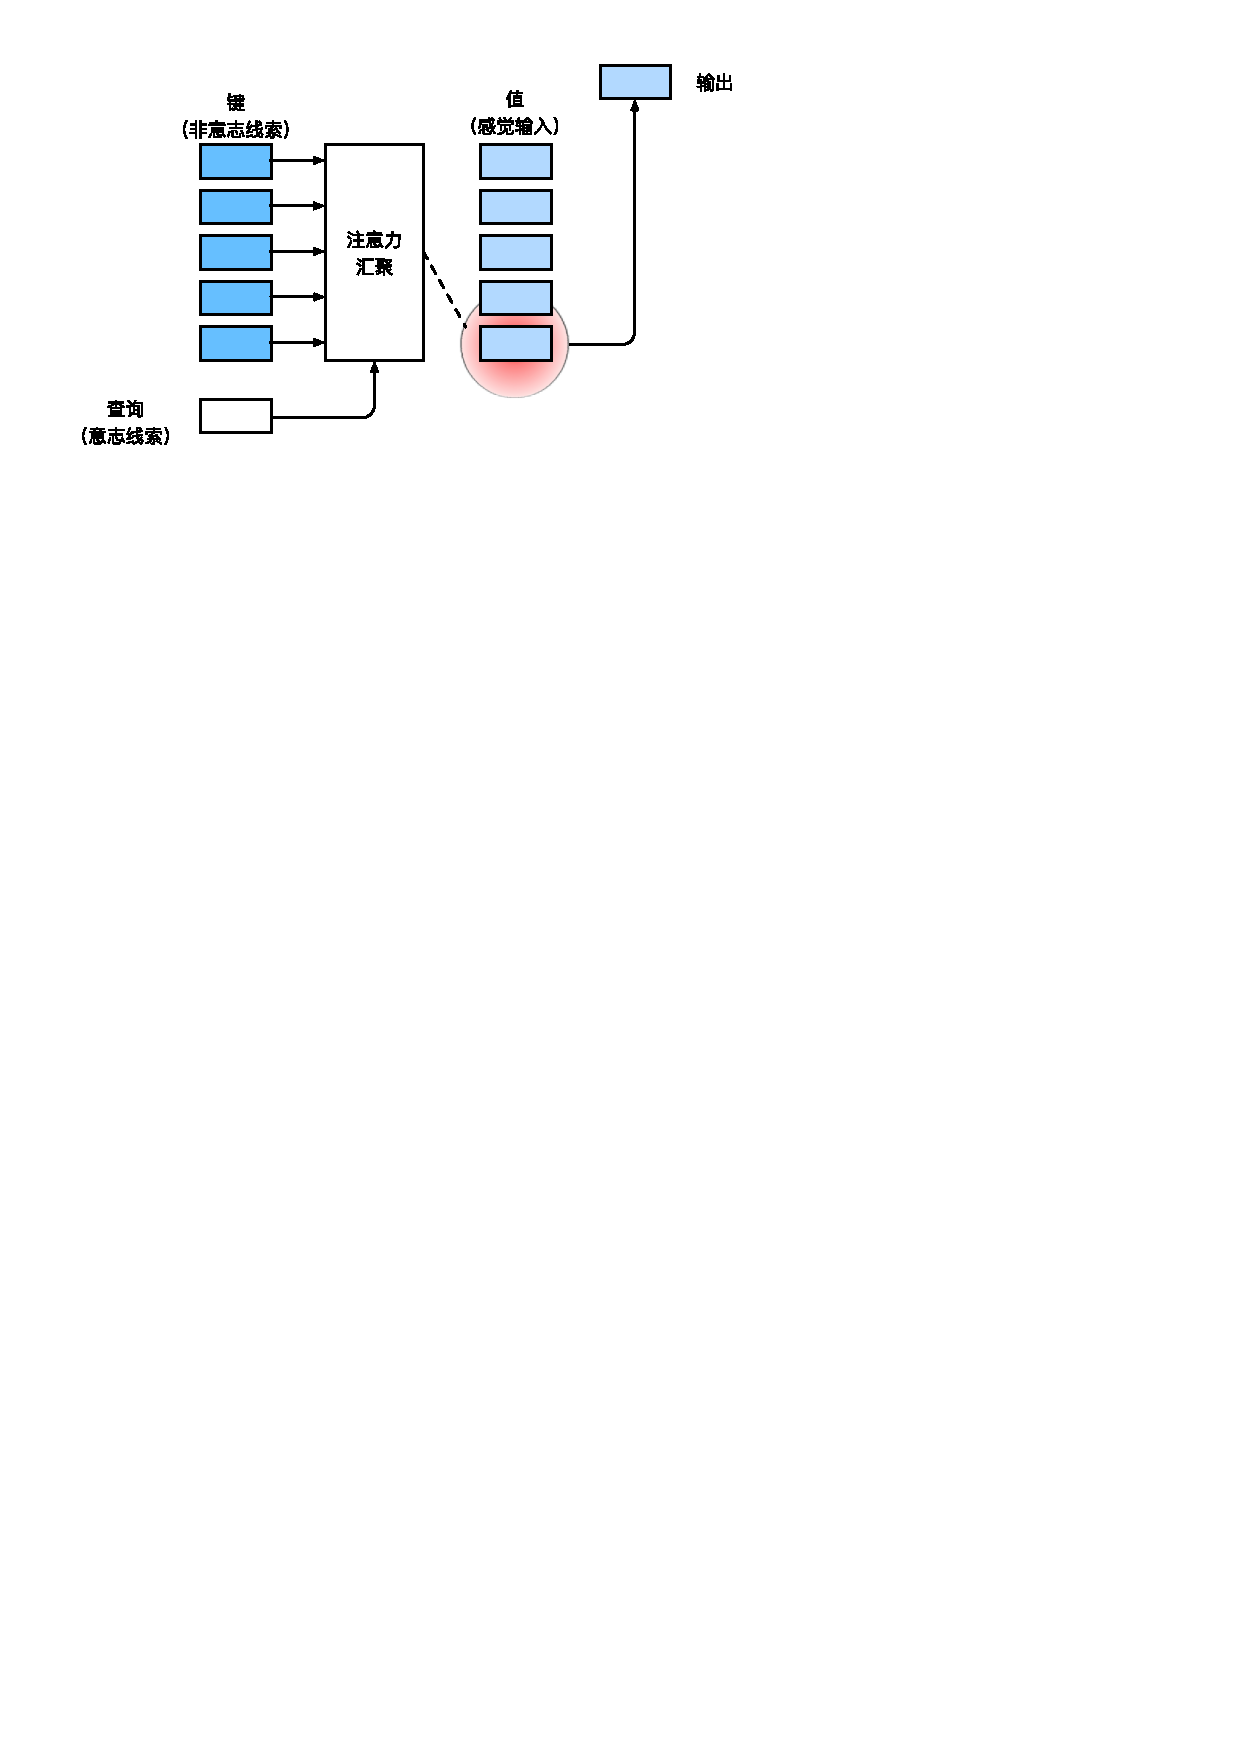
\includegraphics[width=\linewidth, height=0.2\textheight, keepaspectratio]{pic/qkv}
    \caption{注意力机制图示}
    \label{fig:qkv}
  \end{subfigure}
  \hfill
  \begin{subfigure}[b]{0.48\textwidth}
    \centering
    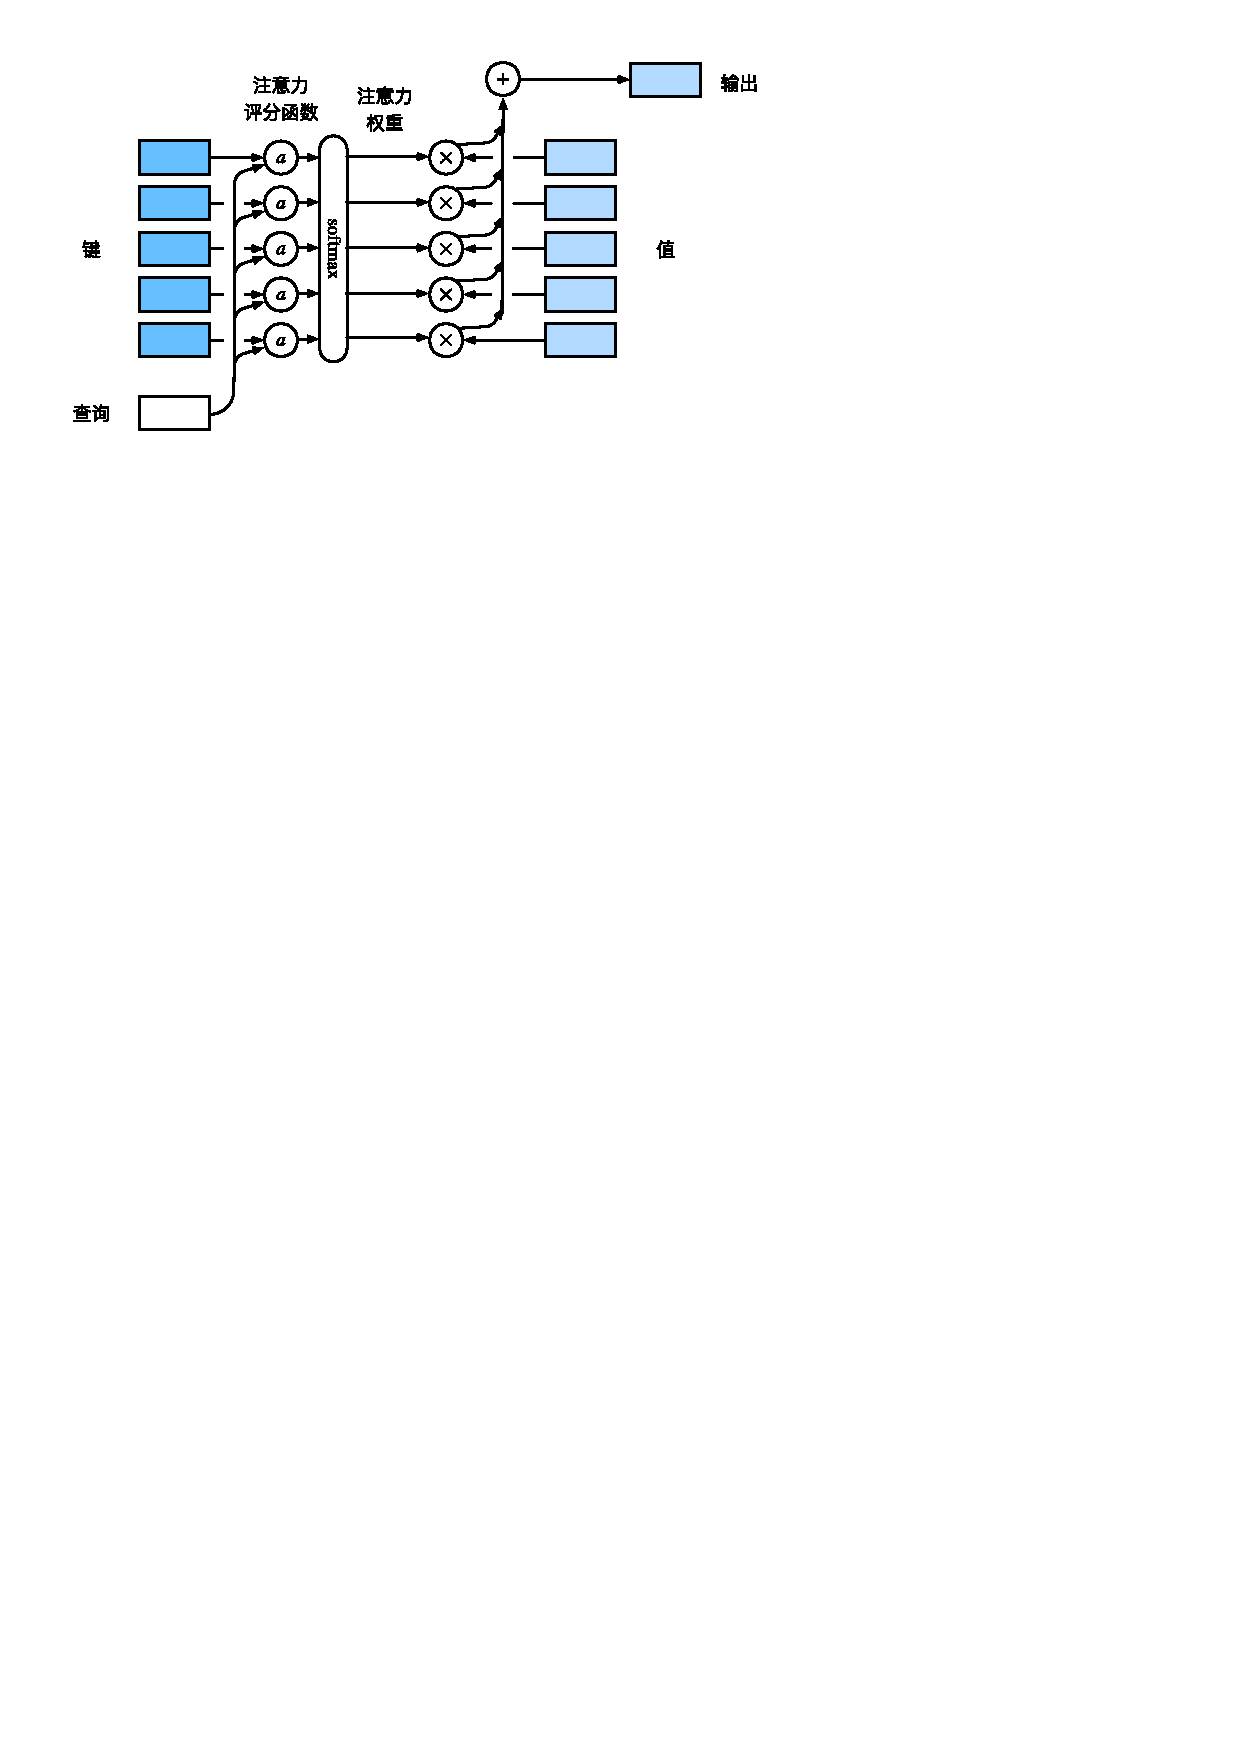
\includegraphics[width=\linewidth, height=0.2\textheight, keepaspectratio]{pic/attention-output}
    \caption{注意力汇聚的输出为值的加权和}
    \label{fig:attention}
  \end{subfigure}
  \caption{注意力机制示意}
  \label{fig:qkv_attention}
\end{figure}
通常用$f\left(\boldsymbol{q}, \boldsymbol{k}, \boldsymbol{v}\right) \in \mathbb{R}$
、$a\left(\boldsymbol{q}, {k}_{i}\right) \in \mathbb{R}$
和$\alpha\left(\boldsymbol{q}, {k}_{i}\right) \in \mathbb{R}$
分别表示注意力汇聚、注意力评分函数和注意力权重，则注意力汇聚函数$f$可表示为值的加权和：
            \begin{equation}
                f\left(\boldsymbol{q}, \boldsymbol{k}, \boldsymbol{v}\right)
                = \sum_{i=1}^{n} \alpha\left(\boldsymbol{q}, {k}_{i}\right) {v}_{i}
                = \sum_{i=1}^{n} \operatorname{softmax}\left(a(\boldsymbol{q}, {k}_{i})\right) {v}_{i}\label{eq:attention-aggregation}
            \end{equation}
\begin{enumerate}[label={（\arabic*）}, leftmargin=2em, labelsep=0.5em, itemsep=0pt]
    \item 当查询和键的长度不同时（不妨设$\boldsymbol{q} \in \mathbb{R}^{q}$、$\boldsymbol{k} \in \mathbb{R}^{k}$），可以使用加性注意力作为评分函数：
    \begin{equation}
a(\boldsymbol{q}, \boldsymbol{k})=\boldsymbol{w}_v^{\top} \tanh \left(\boldsymbol{W}_q \boldsymbol{q}+\boldsymbol{W}_k \boldsymbol{k}\right) \in \mathbb{R}\label{eq:additive-attention}
    \end{equation}
    其中$\boldsymbol{W}_q \in \mathbb{R}^{m \times q}$、$\boldsymbol{W}_k \in \mathbb{R}^{m \times k}$ 和 $\boldsymbol{w}_v \in \mathbb{R}^{m}$ 可学习。
    加性注意力将查询与键分别线性投影后相加，再输入一个仅含单个隐藏层（隐藏单元数为 $m$）且禁用偏置项的感知机；此处 $m$ 为该隐藏层维度，与后文多头注意力中的头数 $h$ 含义不同。
    \item 在点积操作中，设查询和键的维度均为 $d$（在多头注意力中即每个头的键维度 $d_{\text{model}}/h$），且其各分量相互独立、均值为 $0$、方差为 $1$，则两向量点积的均值为 $0$、方差为 $d$。可以通过除以 $\sqrt{d}$ 缩放点积结果，以避免梯度消失或爆炸问题：
        \begin{align}
            &a(\boldsymbol{q}, \boldsymbol{k})=\frac{\boldsymbol{q}^{\top} \boldsymbol{k}}{\sqrt{d}} \in \mathbb{R}
            \Rightarrow
            \operatorname{Attention}(\boldsymbol{Q}, \boldsymbol{K}, \boldsymbol{V})
            = \operatorname{softmax}\left(\frac{\boldsymbol{Q}\boldsymbol{K}^{\top}}{\sqrt{d}}\right) \boldsymbol{V}.
        \end{align}
    \item 掩蔽 softmax 通过将被掩蔽的位置替换为一个极大的负数，从而在 softmax 后将相应的权重压缩为接近 0。这一机制能够有效屏蔽不相关位置，仅关注输入序列中指定范围内的重要信息。
    \begin{figure}[H]
        \centering
        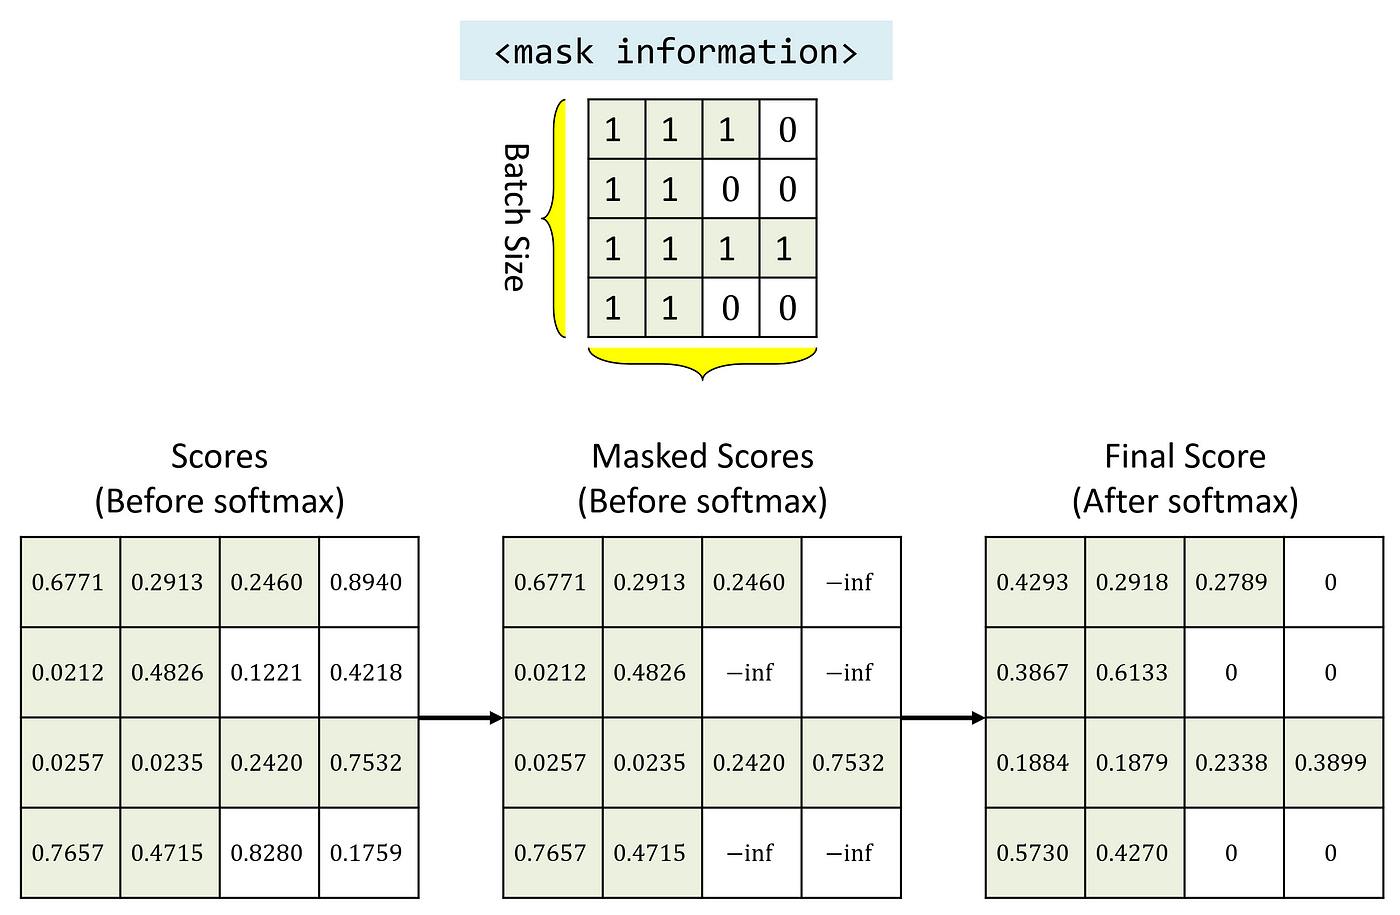
\includegraphics[width=0.6\textwidth, height=0.15\textheight, keepaspectratio]{pic/masked-softmax}
        \caption{掩蔽 softmax，其中任何超出有效长度的位置都被掩蔽并置为 0}
        \label{fig:figure2}
    \end{figure}
    常见的掩码类型包括：
\begin{enumerate}[label={（\alph*）}, leftmargin=2em, labelsep=0.5em, itemsep=0pt]
\item 填充掩码（Padding Mask）：为对齐不同长度的序列，通常在较短序列的末尾添加填充符（padding token）。填充掩码用于在注意力计算中屏蔽这些位置，避免模型关注无效信息。
\item 序列掩码（Sequence Mask）：用于根据任务需求屏蔽输入序列中的特定位置，防止模型处理无效或不相关的信息。例如，在双向模型中，可通过掩码忽略特定上下文，从而更灵活地控制信息流动。
\item 前瞻掩码（Look-ahead Mask）：又称因果掩码（Causal Mask），用于自回归模型中，屏蔽当前位置之后的信息，确保模型仅利用当前位置及之前的输入进行预测，防止未来信息泄漏。
\end{enumerate}
    \item 多头注意力机制通过多个注意力头的并行计算，使模型能够在不同的表示子空间中学习序列中各位置之间的关联，从而在相同注意力结构下捕捉多种范围的依赖关系，提升特征表示的丰富性与建模能力，其结构与计算方式如图~\ref{fig:figure3} 所示。其中第 $i$ 个头通过可学习的投影矩阵 $\boldsymbol{W}_i^{(Q)},\boldsymbol{W}_i^{(K)},\boldsymbol{W}_i^{(V)}$ 将查询、键、值映射到各自的子空间后再计算注意力，各头输出沿特征维度拼接后，由输出投影矩阵 $\boldsymbol{W}^{(O)}$ 融合为最终表示。
    \begin{figure}[H]
      \centering
      \begin{minipage}[c]{0.2\textwidth}
        \centering
        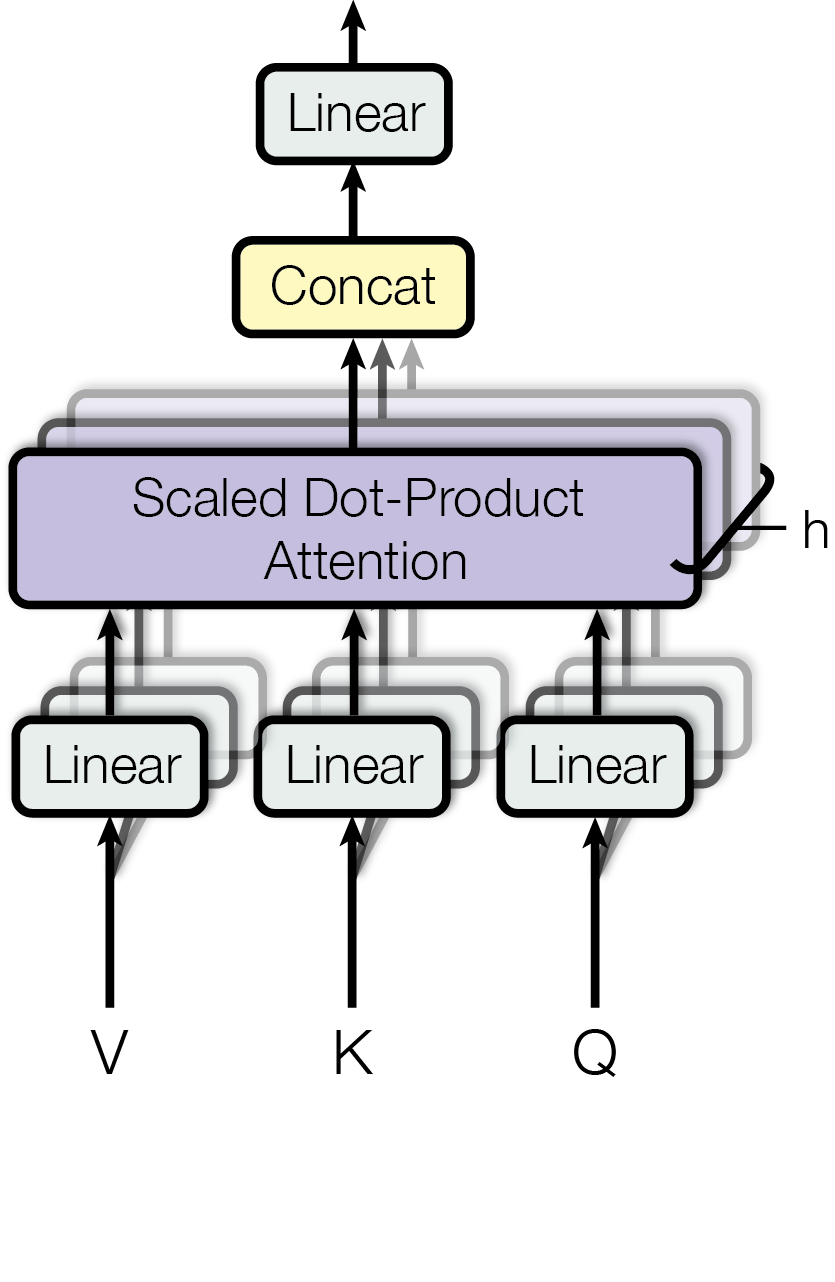
\includegraphics[width=\textwidth, keepaspectratio]{pic/ModalNet-20}
      \end{minipage}%
      \hfill
      \begin{minipage}[c]{0.8\textwidth}
        \begin{align}
          &\text{MultiHead}(\boldsymbol{Q}, \boldsymbol{K}, \boldsymbol{V}) = \text{Concat}(\boldsymbol{h}_1, \dots, \boldsymbol{h}_h)\,\boldsymbol{W}^{(O)}, \\
          &\boldsymbol{h}_{i} = \text{Attention}\left(\boldsymbol{Q}\boldsymbol{W}_{i}^{(Q)}, \boldsymbol{K}\boldsymbol{W}_{i}^{(K)}, \boldsymbol{V}\boldsymbol{W}_{i}^{(V)}\right) \\
          &\text{Attention}(\boldsymbol{Q}, \boldsymbol{K}, \boldsymbol{V}) = \text{softmax}\left(\frac{\boldsymbol{Q} \boldsymbol{K}^{\top}}{\sqrt{d}}\right) \boldsymbol{V}
        \end{align}
      \end{minipage}
      \caption{多头缩放点积注意力}
      \label{fig:figure3}
    \end{figure}
    \item 若查询、键和值均由同一组输入经各自的线性投影得到，则该注意力称为自注意力。记输入序列为 $\boldsymbol{X}$，即取 $\boldsymbol{Q}=\boldsymbol{X}\boldsymbol{W}^{(Q)}$、$\boldsymbol{K}=\boldsymbol{X}\boldsymbol{W}^{(K)}$、$\boldsymbol{V}=\boldsymbol{X}\boldsymbol{W}^{(V)}$；若略去投影、直接以 $\boldsymbol{X}$ 充当查询、键、值，则可简化表示为：
    \begin{equation}
        \text{Attention}\left(\boldsymbol{X}, \boldsymbol{X}, \boldsymbol{X}\right) =\text{softmax}\left(\frac{\boldsymbol{X} \boldsymbol{X}^{\top}}{\sqrt{d}}\right) \boldsymbol{X}
    \end{equation}
    \item 为了使模型能够利用序列的顺序，可通过在输入嵌入中添加位置编码来引入绝对或相对的位置信息。
    位置编码可以通过学习得到，也可以直接固定得到。
    以正余弦位置编码这一固定位置编码方式为例，假设$\boldsymbol{X} \in \mathbb{R}^{n \times d}$表示一个序列中$n$个位置（如$n$个词元）的$d$维嵌入表示，则位置编码使用相同形状的位置嵌入矩阵$\boldsymbol{P} \in \mathbb{R}^{n \times d}$，输出
    $\boldsymbol{X}+ \boldsymbol{P}$，其中：
    \begin{align}
    PE_{pos,2i}&=\sin\left( pos/10000^{2i/d}\right), \quad PE_{pos,2i+1}&=\cos\left( pos/10000^{2i/d}\right)
    \end{align}
\end{enumerate}

\subsubsection{经典Transformer架构}
Transformer 模型由多个编码器（Encoder）和解码器（Decoder）模块交替堆叠而成，其中编码器负责对输入序列进行建模，提取全局特征；解码器则在此基础上生成目标输出序列。
\begin{figure}[H]
    \centering
    \begin{subfigure}[b]{0.5\textwidth}
        \centering
        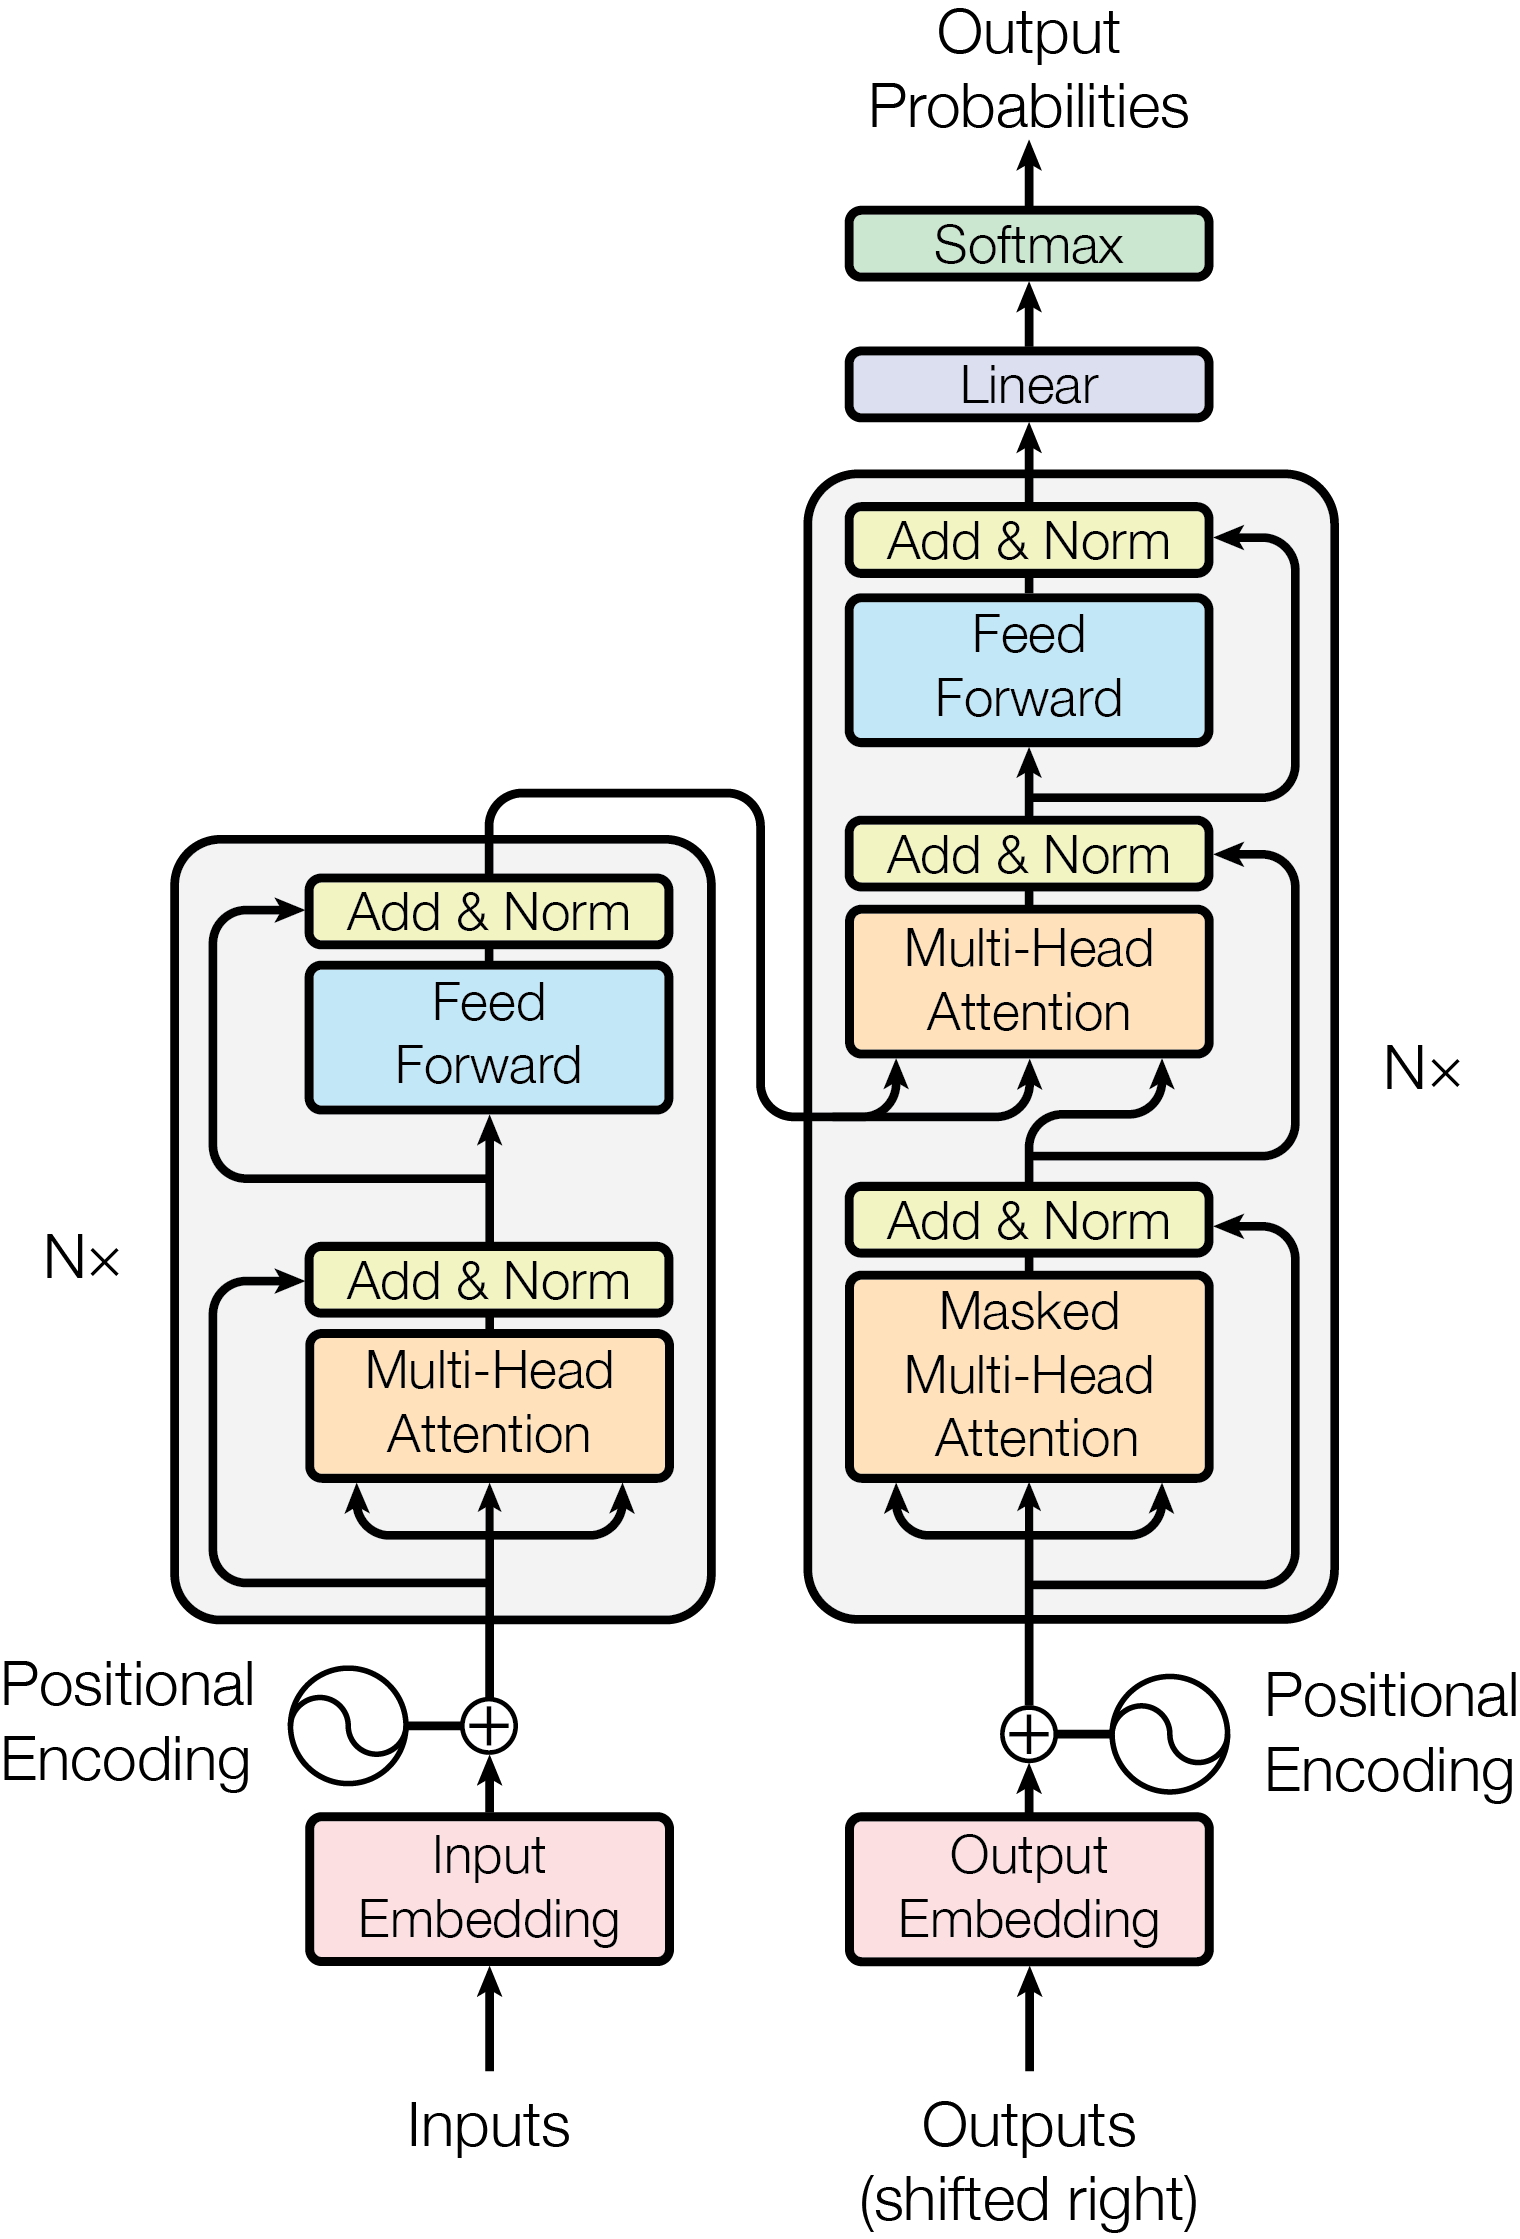
\includegraphics[width=\linewidth, height=0.3\textheight, keepaspectratio]{pic/ModalNet-21}
        \caption{Transformer 整体架构}
        \label{fig:transformer-arch}
    \end{subfigure}
    \hfill
    \begin{subfigure}[b]{0.48\textwidth}
        \centering
        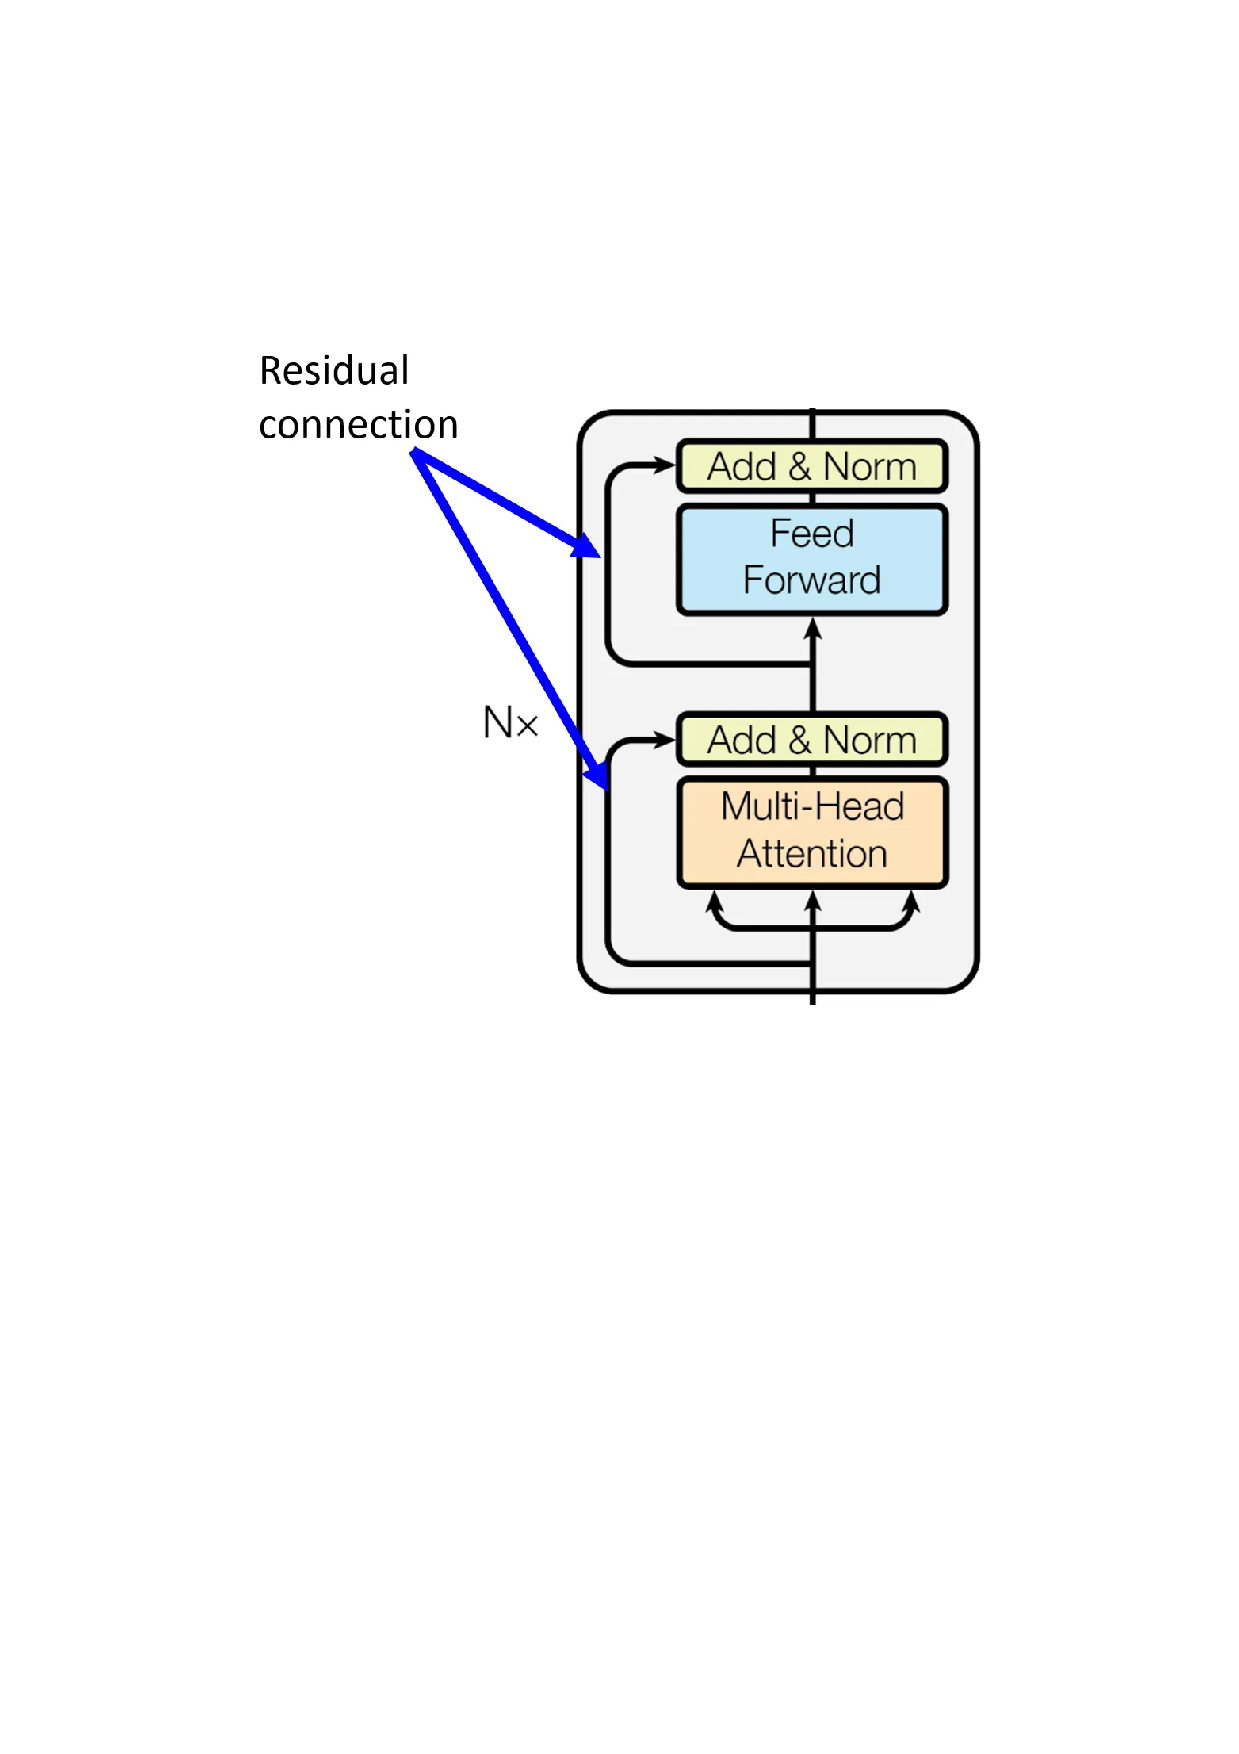
\includegraphics[width=\linewidth, height=0.3\textheight, keepaspectratio]{pic/residual_connection}
        \caption{残差连接}
        \label{fig:residual}
    \end{subfigure}
    \caption{Transformer 架构与残差连接}
    \label{fig:transformer}
\end{figure}
编码器的每一层主要由两部分构成：多头自注意力（Multi-head Self-Attention）机制和基于位置的前馈神经网络（Position-wise Feed-Forward Network）。

解码器则在保留上述结构的基础上，额外引入编码器-解码器注意力（Encoder-Decoder Attention）机制，以实现对编码器输出的动态关注，从而更有效地建模输入与输出之间的对齐关系。

对于Transformer模型中涉及的多种注意力，其查询（Query）、键（Key）和值（Value）的来源分别如表\ref{tab:attn-structure-simple}所示：
\begin{table}[H]
    \centering
    \caption{Transformer 中各注意力模块的输入结构}
    \begin{tabular}{ccc}
        \toprule
        \textbf{模块} & \textbf{注意力类型} & \textbf{Query / Key / Value 的来源} \\
        \midrule
        编码器 & 多头自注意力 & 编码器前一层的输出 / 同 / 同 \\
        解码器 & 掩蔽自注意力 & 解码器前一层的输出 / 同 / 同 \\
        解码器 & 编码器-解码器注意力 & 解码器前一层的输出 / 编码器的输出 / 同 \\
        \bottomrule
    \end{tabular}
    \label{tab:attn-structure-simple}
\end{table}
\begin{enumerate}[label={（\arabic*）}, leftmargin=2em, labelsep=0.5em, itemsep=0pt]
    \item 编码器中的多头自注意力（Multi-Head Self-Attention）：每个位置的 Query、Key 和 Value 均源自编码器前一层的输出，允许所有位置并行地相互关注，从而动态融合全局上下文信息。该机制显著增强了序列表示的建模能力，特别适用于捕捉远距离依赖，缓解传统模型在长序列处理中的性能瓶颈。
    \item 解码器中的掩蔽多头自注意力（Masked Multi-Head Self-Attention）：Query、Key 和 Value 同样均源自解码器前一层的输出，但在注意力计算中引入因果掩码（Causal Mask），限制每个位置仅能访问其自身及之前的词元，从而保留序列生成的自回归特性，防止未来信息泄漏，确保生成过程的因果一致性。
    \item 编码器-解码器注意力（Encoder-Decoder Attention / Cross-Attention）：该模块的 Query 来自解码器前一层的输出，而 Key 与 Value 来自编码器的最终输出。通过跨序列的注意力机制，解码器能够有条件地聚合编码器提取的输入序列（如图像或源语言）的全局语义，实现输入与输出之间的信息对齐与语义桥接，是 Transformer 中连接编码器与解码器的关键枢纽。
\end{enumerate}
在编码器和解码器中，每个子层均采用了残差连接（Residual Connection）和层归一化（Layer Normalization），具体如下：

\begin{enumerate}[label={（\arabic*）}, leftmargin=2em, labelsep=0.5em, itemsep=0pt]
\item 残差连接：通过引入残差映射缓解深层网络训练中的退化问题。对于序列中任意位置的输入向量 $\boldsymbol{x} \in \mathbb{R}^{d}$，子层输出需满足 $sublayer(\boldsymbol{x}) \in \mathbb{R}^{d}$，以保证残差连接 $\boldsymbol{x} + sublayer(\boldsymbol{x})$ 的维度一致，仍属于 $\mathbb{R}^{d}$。

\item 层归一化：在完成残差加法操作后，沿特征维度对结果进行归一化，有助于稳定训练并加快收敛速度，输出 $\text{LayerNorm}(\boldsymbol{x} + sublayer(\boldsymbol{x})) \in \mathbb{R}^{d}$

\end{enumerate}
逐位前馈网络对序列中所有位置的表示独立地应用同一带偏置的多层感知机\supercite{vaswaniAttentionAllYou2017}：
    \begin{equation}
        FFN(\boldsymbol{x}) = \boldsymbol{W}_{2} \max(0, \boldsymbol{W}_{1} \boldsymbol{x} + \boldsymbol{b}_{1}) + \boldsymbol{b}_{2}
    \end{equation}
\subsection{经典Vision Transformer}
起初，尽管 Transformer 在自然语言处理领域取得了显著成果，其在计算机视觉中的应用相对有限。在早期的视觉任务中，注意力机制通常作为辅助模块嵌入卷积神经网络（Convolutional Neural Network, CNN）架构，或仅替代其部分组件，整体结构仍以卷积为主导。

Vision Transformer（ViT） 的提出打破了这一范式限制。Dosovitskiy 等人首次在 ImageNet 数据集上成功地将经典的 Transformer 架构直接应用于图像分类任务，提出了 ViT 模型\supercite{dosovitskiyImageWorth16x162021}。该方法将输入图像划分为一系列固定大小的图像块（patches），对每个图像块进行线性投影并添加位置编码后构建为序列输入，使 Transformer 能够以类似处理文本序列的方式对图像进行建模。

该实验结果表明，ViT 在图像分类任务中不仅可达到与传统 CNN 相当的性能，在大规模数据集与充分训练的条件下，还因其能够同时建模局部与全局依赖关系，故展现出更强的表达能力与泛化性能。

本文将 ViT 用作视觉编码器，以服务于数学表达式图像到 LaTeX 的序列生成任务。为此，本节先系统阐述 ViT 将图像转化为序列并经 Transformer 编码的核心思想与基本架构，再说明其编码器输出在图像分类与序列生成两类任务中的不同使用方式，从而引出本文所采用的编码方案。
\begin{figure}[H]
    \centering
    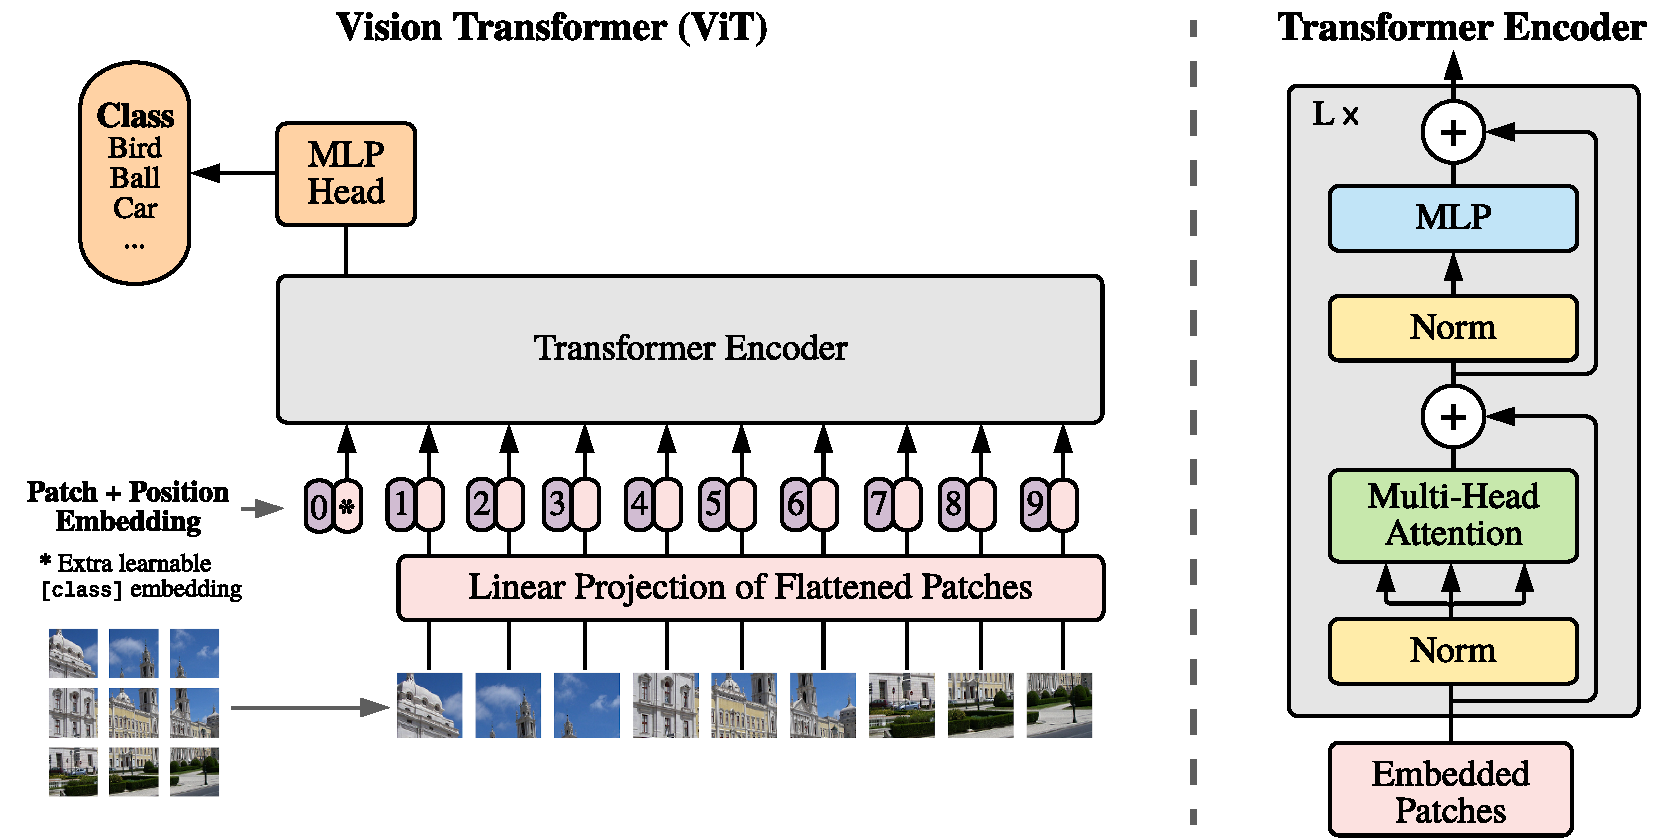
\includegraphics[width=0.8\textwidth, height=0.3\textheight, keepaspectratio]{pic/model_scheme}
    \caption{Vision Transformer 架构示意图}
    \label{fig:vit-architecture}
\end{figure}
Vision Transformer（ViT）的核心思想是将输入图像划分为一系列固定大小且不重叠的图像块（如 $16 \times 16$ 或 $32 \times 32$ 像素），
并将每个图像块展平后通过线性映射嵌入到一个低维表示空间。
随后，为每个块添加可学习的位置编码以保留空间位置信息。
通常在嵌入序列的前端插入一个可学习的 [CLS] 标记，作为可选的全局聚合位置；其末层表示的具体用途取决于下游任务，将在后文按任务类型分别说明。

这种基于图像块的表示方法使模型能够在保留局部空间结构的基础上，借助自注意力机制建模整幅图像中的全局依赖关系。

下面将结合图 \ref{fig:vit-architecture}，按照数据流动的顺序，对 Vision Transformer 的整体架构及其数据传递过程进行详细介绍：
\begin{enumerate}[label={（\arabic*）}, leftmargin=2em, labelsep=0.5em, itemsep=0pt]
\item 图像展平（Flattening）：
将输入图像 $\boldsymbol{x} \in \mathbb{R}^{H \times W \times C}$ 按照大小为 $P \times P$ 的不重叠区域划分为 $N = \frac{HW}{P^2}$ 个图像块（patch），其中 $H \times W$ 为图像分辨率，$C$ 为通道数，$P$ 为每个块的边长。

对每个图像块按空间位置展开其所有像素通道值，展平成一维向量，得到 $N$ 个向量 $\boldsymbol{x}_p^i \in \mathbb{R}^{P^2 \cdot C}$。
将这些展平后的块向量按其原始空间顺序排列，组成二维块序列，即为：
\[
\boldsymbol{x}_{p} = [\boldsymbol{x}_p^1, \boldsymbol{x}_p^2, \ldots, \boldsymbol{x}_p^N] \in \mathbb{R}^{N \times (P^2 \cdot C)},
\]
其中$\boldsymbol{x}_p^i$ 表示第 $i$ 个图像块的展平表示。

该二维块序列经下述线性投影、类别标记与位置编码处理后，才构成 Transformer 编码器的实际输入 $\boldsymbol{z}_0$。
    \item 图像块的线性投影（Linear Projection of Flattened Patches）：由于 Transformer 所有层保持固定的潜空间维度 $D$，需通过可学习的线性投影将每个图像块嵌入到 $D$ 维空间，得到由$N$个图像块组成的嵌入序列：
    \begin{equation}
        \left[\boldsymbol{x}_p^1 \boldsymbol{E}; \cdots ; \boldsymbol{x}_p^N \boldsymbol{E}\right] \in \mathbb{R}^{N \times D}, \quad \boldsymbol{E} \in \mathbb{R}^{(P^2 \cdot C) \times D}.
    \end{equation}
    \item 添加类别标记与位置编码（Patch + Position Embedding）：
    \begin{enumerate}[label={（\alph*）}, leftmargin=2em, labelsep=0.5em, itemsep=0pt]
\item 类别标记（[CLS] Token）：在嵌入序列前添加一个可学习的向量 $\boldsymbol{x}_{\text{class}}$，作为分类标记（[CLS] token），构成输入序列的首位，即：
\begin{equation}
    \left[\boldsymbol{x}_{\text{class}}; \boldsymbol{x}_p^1 \boldsymbol{E}; \cdots ; \boldsymbol{x}_p^N \boldsymbol{E}\right] \in \mathbb{R}^{\left(N+1\right) \times D}.
\end{equation}
    \item 位置编码：为保持块序列的位置信息，向每个块嵌入添加可学习的一维位置编码，构成 Transformer 的最终输入序列，即：
    \begin{equation}
        \boldsymbol{z}_0 = \left[\boldsymbol{x}_{\text{class}}; \boldsymbol{x}_p^1 \boldsymbol{E}; \cdots ; \boldsymbol{x}_p^N \boldsymbol{E}\right] + \boldsymbol{E}_{\text{pos}}, \quad \boldsymbol{E}_{\text{pos}} \in \mathbb{R}^{(N+1) \times D}.
    \label{eq:pos-emb}
    \end{equation}
    \end{enumerate}
    \item Transformer 编码器（Transformer Encoder）：由交替 $L$ 次的多头自注意力（Multi-Head Self-Attention, MSA）和多层感知机（Multi-Layer Perceptron, MLP）构成。
    每个子层前应用了层归一化（Layer Normalization，LN)，每个子层之后通过残差连接（Residual Connection）与输入相加，形成输出。

    多头自注意力（MSA）和多层感知机（MLP）在 Transformer 编码器中的每层计算过程如式\ref{eq:transformer-encoder-msa}和式\ref{eq:transformer-encoder-mlp}所示（含层归一化和残差连接）：
    \begin{align}
        \boldsymbol{z}'_l &= \text{MSA}(\text{LN}(\boldsymbol{z}_{l-1})) + \boldsymbol{z}_{l-1}, \qquad l = 1, 2, \dots, L \label{eq:transformer-encoder-msa} \\
        \boldsymbol{z}_l &= \text{MLP}(\text{LN}(\boldsymbol{z}'_l)) + \boldsymbol{z}'_l, \qquad l = 1, 2, \dots, L \label{eq:transformer-encoder-mlp}
    \end{align}
    其中 MLP 模块包含两个线性层与一个 GELU 激活函数，后者的形式为：
    \begin{equation}
        \text{GELU}(x) = x \cdot \Phi(x) = x \cdot \frac{1}{2} \left[1 + \text{erf}\left(\frac{x}{\sqrt{2}}\right)\right],
        \label{eq:GELU}
    \end{equation}
    其中 $\Phi(\cdot)$ 为标准正态分布 $\mathcal{N}(0,1)$ 的累积分布函数（CDF），$\operatorname{erf}(\cdot)$ 为误差函数。
    \item 编码器输出（Encoder Output）：经过 $L$ 层编码后，编码器输出一组与输入词元一一对应的末层表示 $\{\boldsymbol{z}^{0}_L, \boldsymbol{z}^{1}_L, \dots, \boldsymbol{z}^{N}_L\}$，其中 $\boldsymbol{z}^{0}_L$ 对应 [CLS] 标记，$\boldsymbol{z}^{1}_L, \dots, \boldsymbol{z}^{N}_L$ 对应各图像块。在每一层的多头自注意力中，所有词元相互交互，使每个表示都融合了局部图像块特征与全局上下文信息。
\end{enumerate}

ViT 编码器本身只完成对图像的特征提取，其输出表示的使用方式取决于具体的下游任务。下面分别说明两类典型任务对应的处理方式。

\textbf{（1）图像分类任务。} 取 [CLS] 标记的末层表示 $\boldsymbol{z}^{0}_L$ 作为整幅图像的全局表征——在逐层自注意力中，[CLS] 标记持续聚合所有图像块的语义信息，故可代表全图；将其经层归一化后送入分类头（MLP Head），即得到类别预测：
\begin{equation}
\boldsymbol{y} = \text{LN}(\boldsymbol{z}^{0}_L), \qquad
\hat{\boldsymbol{y}} = \text{MLP}(\boldsymbol{y}),
\end{equation}
其中 $\hat{\boldsymbol{y}} \in \mathbb{R}^{C}$ 为图像在 $C$ 个类别上的预测得分（logits），经 Softmax 归一化后得到类别概率分布，$C$ 为类别总数；分类头通常由一至两层全连接网络构成，并结合非线性激活与 Dropout。这正是 Dosovitskiy 等人提出的经典 ViT 所采用的输出方式。

\textbf{（2）序列生成任务。} 此类任务（如图像描述、图像到 LaTeX 转换）需要输出一个变长的词元序列而非单一类别，因此不使用面向全局聚合的 [CLS] 标记与分类头，而是保留全部图像块的末层表示 $\{\boldsymbol{z}^{1}_L, \dots, \boldsymbol{z}^{N}_L\}$ 作为图像的特征序列，交由自回归解码器生成目标序列：解码器在交叉注意力中以该特征序列为键（Key）与值（Value）、以已生成的词元为查询（Query），循环预测下一个词元，直至生成终止符。本文的数学表达式图像到 LaTeX 转换任务即属此类，采用 ViT 编码器与 Transformer 解码器相结合的结构；该“编码器—解码器”结构的具体设计与实现将在“模型构建”一章详细展开。

  \newpage\section{训练原理}
\subsection{评价指标}
\subsubsection{交叉熵损失函数与准确率}
为全面评估模型在 LaTeX 序列生成过程中的训练效果与预测性能，引入损失层面与性能层面的两类指标：
交叉熵损失（Cross-Entropy Loss，以整数标签为输入）与逐词元准确率（Token-Level Accuracy）。
前者作为优化目标，衡量每个位置上预测分布与真实标签之间的差异；
后者作为性能指标，统计生成序列中预测词元与参考词元的匹配情况，从而反映模型在序列级别的预测精度。
\begin{enumerate}[label={（\arabic*）}, leftmargin=2em, labelsep=0.5em, itemsep=0pt]
    \item 交叉熵损失函数：
    模型在某一时间步的输出为 logit 向量 $\boldsymbol{z} = [z_0, z_1, \dots, z_{C-1}]$，其中 $C$ 为类别总数，$z_j$ 表示第 $j$ 类的预测得分（未归一化），真实标签为 $y \in \{0, 1, \dots, C{-}1\}$。则该时间步的交叉熵损失定义为：
    \begin{equation}
    \mathcal{L}_{\text{CE}} = -\log \left( \frac{e^{z_{y}}}{\sum_{j=0}^{C-1} e^{z_j}} \right) = -z_{y} + \log\left( \sum_{j=0}^{C-1} e^{z_j} \right)
    \end{equation}
    上式右端将 Softmax 与负对数似然合并为对数-求和-指数（log-sum-exp）形式，可直接以未归一化的 logits 计算，避免显式指数运算导致的上溢／下溢等数值不稳定问题。该损失函数在 PyTorch 中通过如下函数实现：
    \begin{center}
        \texttt{torch.nn.functional.cross\_entropy(logits, labels)}
    \end{center}
    其中 \texttt{labels} 为整数编码的真实标签张量，\texttt{logits} 为模型输出的未归一化得分张量；
    该实现内部融合了 log-softmax 与负对数似然计算，保证数值稳定性。
    \item 准确率：
    准确率用于衡量模型在所有预测位置上分类正确的比例。模型在每个位置的预测类别为：
    \begin{equation}
    \hat{y} = \arg\max_{j} z_j
    \end{equation}
    整体准确率定义为：
    \begin{equation}
    \text{Accuracy} = \frac{1}{N} \sum_{i=1}^{N} \mathbb{I}[\hat{y}_i = y_i]
    \end{equation}
    其中 $\mathbb{I}[\cdot]$ 为指示函数，表示预测是否正确，$N$ 为所有评估位置的总数。
\end{enumerate}
\subsubsection{掩蔽损失函数与掩蔽准确率}
    为满足批量训练对张量形状一致性的要求（解码器的位置嵌入亦需预设固定的最大长度），需对标签序列进行填充，统一长度至最大值。填充标记通常为特殊符号 \texttt{<PAD>}，其对应的标签值设为 $0$。为避免这些填充位置对损失计算与评估指标造成干扰，引入掩蔽机制，在损失与准确率计算中仅考虑非填充位置。
    加权平均的掩蔽交叉熵损失函数定义如下：
    \begin{equation}
    \mathcal{L}_{\text{masked}} = \frac{\sum_{i=1}^{L} m_i \cdot \mathcal{L}_i}{\sum_{i=1}^{L} m_i}, \quad
    m_i =
    \begin{cases}
    1, & \text{若 } y_i \neq 0 \text{ 且 } \mathcal{L}_i < 10^8 \\
    0, & \text{否则}
    \end{cases}
    \end{equation}
    其中，$L$ 表示序列长度，$y_i$ 为第 $i$ 个时间步的真实标签，$\mathcal{L}_i$ 为其对应的单步交叉熵损失，$m_i$ 为掩码指示变量。仅当 $y_i$ 为有效标签（非 \texttt{<PAD>}）且 $\mathcal{L}_i$ 不出现数值异常时，才将该位置纳入最终损失计算。
    掩蔽准确率同样排除填充位置，仅在非填充位置统计预测是否正确；与掩蔽损失不同的是，准确率\textbf{不}额外排除 $\mathcal{L}_i \ge 10^8$ 的位置，故测试集中被映射为 \texttt{[UNK]} 的词表外（OOV）目标位置仍计入统计——由于 \texttt{[UNK]} 在输出层被一项词频先验偏置（其设计见“模型构建”一章的 TokenOutput 层）禁止生成，这些位置必然计为错误，因而所报告的准确率对该类位置取了偏保守的估计。
\subsubsection{Levenshtein 距离与BLEU-4 分数}
为全面评估模型生成的 LaTeX 序列与参考标签序列之间的输出质量，引入字符级别与片段级别的两类指标：Levenshtein 距离与 BLEU 分数。
前者关注最小编辑路径，主要衡量结构差异；后者基于 $n$-gram 匹配，评估语言模式的一致性。
\begin{enumerate}[label={（\arabic*）}, leftmargin=2em, labelsep=0.5em, itemsep=0pt]
    \item Levenshtein 距离（编辑距离）：衡量将预测序列 $a$ 转换为参考序列 $b$ 所需的最小编辑操作数，包括字符的插入、删除与替换。该指标可度量生成输出与标签之间的字符级结构差异，递归定义如下：
    \begin{equation}
    \operatorname{lev}(a, b) =
    \begin{cases}
        |a|, & \text{若 } |b| = 0 \\
        |b|, & \text{若 } |a| = 0 \\
        \operatorname{lev}(\operatorname{tail}(a), \operatorname{tail}(b)), & \text{若 } \operatorname{head}(a) = \operatorname{head}(b), \\
        1 + \min\left\{
            \begin{array}{l}
                \operatorname{lev}(\operatorname{tail}(a), b) \\
                \operatorname{lev}(a, \operatorname{tail}(b)) \\
                \operatorname{lev}(\operatorname{tail}(a), \operatorname{tail}(b))
            \end{array}
        \right., & \text{否则}
    \end{cases}
    \end{equation}
    其中，$\operatorname{head}(a)$ 表示字符串 $a$ 的首字符，$\operatorname{tail}(a)$ 表示其余子串。例如，
    若 $a = \texttt{\textbackslash sqrt}$，则 $\operatorname{head}(a) = \texttt{\textbackslash}$，$\operatorname{tail}(a) = \texttt{sqrt}$。
    为便于跨样本比较，实际使用时可采用归一化编辑距离，即将 $\operatorname{lev}(a,b)$ 除以参考序列长度 $|b|$ 后在测试集上取平均，其取值范围为 $[0,1]$，数值越小表示生成结果与参考序列越接近。编辑距离与 BLEU 从不同侧面刻画生成质量且高度相关；为避免指标冗余，本文实验以 BLEU-4 作为序列生成质量的主要报告指标，编辑距离仅作为概念参照。
\item BLEU-4 分数：该指标广泛用于自然语言生成任务，用以评估生成序列在词片段（$n$-gram）层面与参考序列之间的语言模式一致性。BLEU-4 综合考虑了从 $1$-gram 到 $4$-gram 的匹配情况，并引入长度惩罚机制，防止模型生成明显短于参考答案的序列。其计算公式如下：
\begin{align}
&\text{BP} =
\begin{cases}
1, & \text{若 } |P| > |G|, \\
\exp\left(1 - \frac{|G|}{|P|}\right), & \text{若 } |P| \leq |G|.
\end{cases} \\
&\text{BLEU-4} = \text{BP} \cdot \exp\left( \sum_{n=1}^{4} w_n \log p_n \right).
\end{align}
其中，$|P|$ 与 $|G|$ 分别表示生成序列与有效参考序列的长度，$p_n$ 表示 $n$-gram 的精确匹配率，$w_n$ 为对应的加权系数，通常取 $w_n = \frac{1}{4}$。$\text{BP}$ 为简短惩罚项（brevity penalty），当生成序列明显短于参考序列时将对得分进行指数衰减，以避免不完整输出带来高评分。

需要注意的是，当生成序列较短或某阶 $n$-gram 完全无匹配时，存在 $p_n = 0$ 导致整体得分坍缩为 $0$ 的问题。为此，本文在计算 BLEU-4 时采用平滑方法（smoothing method 1），对零计数的高阶 $n$-gram 匹配率施加微小正值修正，使得分能够平滑地反映部分匹配的质量。此外，LaTeX 词元具有大小写敏感性（如 \texttt{\textbackslash Gamma} 与 \texttt{\textbackslash gamma} 表示不同符号），故计算时按空白切分词元且不做任何大小写归一化，并剔除 \texttt{[START]}/\texttt{[END]} 特殊标记。
\end{enumerate}
\subsection{优化算法}
\subsubsection{随机梯度下降法(SGD)}
在深度学习中，目标函数通常是训练数据集中每个样本的损失函数的平均值。
若给定$n$个样本的训练数据集，假设$f_i(\boldsymbol{x})$是第$i$个训练样本的损失函数，其中$\boldsymbol{x}$
是参数向量，则目标函数$f(\boldsymbol{x})$可以表示为所有样本损失函数的平均值：
\begin{equation}
    f(\boldsymbol{x})=\frac{1}{n} \sum_{i=1}^n f_i(\boldsymbol{x}).
\end{equation}
目标函数$f(\boldsymbol{x})$的梯度可计算为：
\begin{equation}
    \nabla f(\boldsymbol{x})=\frac{1}{n} \sum_{i=1}^n \nabla f_i(\boldsymbol{x}).
\end{equation}
如果使用梯度下降法，则每个自变量迭代的计算代价为 $\mathcal{O}(n)$，随着$n$线性增长。

随机梯度下降（Stochastic Gradient Descent, SGD）可将每次迭代的计算代价从梯度下降的 $\mathcal{O}(n)$ 降至常数 $\mathcal{O}(1)$。

在随机梯度下降的每次迭代中，对数据样本随机均匀采样一个索引 $i$，其中 $i \in\{1, \ldots, n\}$，
计算梯度 $\nabla f_i(\boldsymbol{x})$ 以更新 $\boldsymbol{x}$：
\begin{align}
    \boldsymbol{x} & \leftarrow \boldsymbol{x}-\eta \nabla f_i(\boldsymbol{x}),\\
    \mathbb{E}_{i} \nabla f_i(\boldsymbol{x}) & =\frac{1}{n} \sum_{i=1}^n \nabla f_i(\boldsymbol{x}) = \nabla f(\boldsymbol{x}),
\end{align}
其中$\eta$是学习率。\supercite{zhang2023dive}

\subsubsection{AdamW优化算法}
AdamW 保留了 Adam 自适应一阶与二阶矩估计的优势，同时将权重衰减项显式从梯度更新中解耦，从而实现了更纯粹的正则化过程，
有效缓解了原始 Adam 在 L2 正则下的性能退化问题。
相较于 SGD，AdamW 通常收敛更快、对学习率与初始化更鲁棒，其解耦式权重衰减在 Transformer 类模型的训练中应用广泛。
\supercite{loshchilovDecoupledWeightDecay2019a}

以下为 AdamW 算法伪代码。与采用 L2 正则的 Adam 相比，其关键差异在于：权重衰减项 $\lambda\boldsymbol{\theta}_{t-1}$ 不再并入梯度 $\boldsymbol{g}_t$（因而不参与一阶、二阶矩的估计），而是被解耦至参数更新步中直接作用于权重，该差异已用\fcolorbox{red}{white}{红色框}标注。
\begin{algorithm}[H]
\caption{AdamW 优化算法（Adam with Decoupled Weight Decay）}
\KwIn{学习率 $\alpha=0.001$（此为 Adam/AdamW 通用默认值，本文实际取值见式后说明），权重衰减系数 $\lambda$，一阶矩衰减率 $\beta_1=0.9$，二阶矩衰减率 $\beta_2=0.999$，数值稳定项 $\epsilon=10^{-8}$}
\KwIn{初始参数 $\boldsymbol{\theta}_0 \in \mathbb{R}^n$，一阶矩向量 $\boldsymbol{m}_0 \leftarrow \boldsymbol{0}$，二阶矩向量 $\boldsymbol{v}_0 \leftarrow \boldsymbol{0}$，时间步 $t \leftarrow 0$，学习率调度器倍率 $\eta_0 \in \mathbb{R}$}
\KwOut{最终优化参数 $\boldsymbol{\theta}_t$}
\BlankLine
\While{未满足停止条件}{
    $t \leftarrow t + 1$\;
    $\nabla f_t\left(\boldsymbol{\theta}_{t-1}\right) \leftarrow \text{SelectBatch}(\boldsymbol{\theta}_{t-1})$ \tcp*{计算当前批次的梯度}
    $\boldsymbol{g}_t \leftarrow \nabla f_t\left(\boldsymbol{\theta}_{t-1}\right)$ \tcp*{仅计算梯度；权重衰减已解耦，不在此处加入}
    $\boldsymbol{m}_t \leftarrow \beta_1 \boldsymbol{m}_{t-1} + (1 - \beta_1)\boldsymbol{g}_t$ \tcp*{更新一阶矩估计}
    $\boldsymbol{v}_t \leftarrow \beta_2 \boldsymbol{v}_{t-1} + (1 - \beta_2)(\boldsymbol{g}_t \odot \boldsymbol{g}_t)$ \tcp*{更新二阶矩估计}
    $\hat{\boldsymbol{m}}_t \leftarrow \boldsymbol{m}_t / (1 - \beta_1^t)$ \tcp*{一阶矩偏差校正}
    $\hat{\boldsymbol{v}}_t \leftarrow \boldsymbol{v}_t / (1 - \beta_2^t)$ \tcp*{二阶矩偏差校正}
    $\eta_t \leftarrow \text{SetScheduleMultiplier}(t)$ \tcp*{调整倍率（固定、衰减或重启）}
    $\boldsymbol{\theta}_t \leftarrow \boldsymbol{\theta}_{t-1} - \eta_t \left( \alpha \frac{\hat{\boldsymbol{m}}_t}{\sqrt{\hat{\boldsymbol{v}}_t} + \epsilon} + \fcolorbox{red}{white}{$\lambda \boldsymbol{\theta}_{t-1}$} \right)$ \tcp*{更新参数，解耦权重衰减}
}
\Return{$\boldsymbol{\theta}_t$}
\end{algorithm}

在本文的训练配置中，伪代码中的学习率调度项 $\eta_t \cdot \alpha$ 采用 Transformer 原论文提出的预热（warmup）策略\supercite{vaswaniAttentionAllYou2017}：
\begin{equation}
    \eta_t \cdot \alpha = d_{\text{model}}^{-0.5} \cdot \min\left(t^{-0.5},\ t \cdot t_{\text{warmup}}^{-1.5}\right),
\end{equation}
其中 $t$ 为训练步数，$d_{\text{model}}$ 为模型嵌入维度。该调度在前 $t_{\text{warmup}}$ 步内使学习率随步数线性增长，避免训练初期自适应矩估计尚不稳定时大学习率导致的发散；此后按 $1/\sqrt{t}$ 衰减，保证训练后期的稳定收敛。学习率峰值出现在 $t = t_{\text{warmup}}$ 处，其大小为 $d_{\text{model}}^{-0.5} \cdot t_{\text{warmup}}^{-0.5}$，即预热步数越小，峰值学习率越高。此外需说明的是，前述 AdamW 算法框中的 $\beta_2=0.999$、$\epsilon=10^{-8}$、$\alpha=0.001$ 为该算法的通用默认值；本文实际采用 Transformer 原论文的配置 $\beta_2=0.98$、$\epsilon=10^{-9}$，且基础学习率 $\alpha$ 由上述预热调度统一接管（实现中以基础学习率 $1.0$ 乘以调度倍率 $\eta_t$），不再单独取 $0.001$。

预热步数需与批大小协同设定：批大小增大后，每轮的优化步数相应减少，若预热步数不变，则预热阶段将占据过大的训练比例，使模型长期处于低学习率状态。本文取 $d_{\text{model}}=256$、$t_{\text{warmup}}=800$（对应峰值学习率约 $2.2\times10^{-3}$）；在批大小 $768$（每轮约 $52$ 个优化步）下，预热在约第 $15$ 轮结束，约占早停时总优化步数（$78$ 轮、约 $4{,}100$ 步）的 $1/5$，兼顾了训练初期的稳定性与适度的预热占比。

\subsubsection{梯度裁剪}
在大批量、强预热的训练设定下，学习率在预热结束附近达到峰值，此时若某一批次产生范数异常的梯度，单步更新即可能将参数推离正常区域并引发不可恢复的训练发散。梯度裁剪（Gradient Clipping）通过限制梯度的全局范数来阻断这一路径：设全体参数梯度拼接所得向量为 $\boldsymbol{g}$，给定阈值 $c$，则裁剪操作为：
\begin{equation}
    \boldsymbol{g} \leftarrow \boldsymbol{g} \cdot \min\left(1,\ \frac{c}{\|\boldsymbol{g}\|_2}\right),
\end{equation}
即当 $\|\boldsymbol{g}\|_2 \le c$ 时梯度保持不变，否则按比例缩放至范数恰为 $c$。该操作只改变异常梯度的幅值而保留其方向，对正常训练步几乎无影响，却为峰值学习率附近的更新提供了硬性保护。本文取 $c=1.0$，在每次反向传播之后、参数更新之前施加该裁剪。梯度裁剪的必要性在本文实验中得到了直接验证（见“结果与评价”一章的训练稳定性分析）。

\subsection{正则化}
\subsubsection{Dropout正则化}
具有大量参数的深度神经网络虽然具备强大的学习能力，但往往容易出现严重的过拟合问题，导致模型在新数据上的泛化能力不足。
为缓解该问题，Srivastava 等人于 2014 年提出了标准的 Dropout 正则化方法\supercite{srivastava2014dropout}。
其核心思想是在模型训练过程中，以一定的概率随机丢弃部分神经元及其连接，从而有效减少神经元之间的共适应性，显著降低过拟合风险。

本节简要介绍 Dropout 神经网络模型的基本原理。设神经网络包含 $L$ 个隐藏层，记 $l \in \{1, \ldots, L\}$ 表示网络的隐藏层索引。
\begin{itemize}
    \item $\boldsymbol{z}^{(l)}, \boldsymbol{y}^{(l)}$：第$l$层的输入向量和输出向量，
    \item $\boldsymbol{W}^{(l)}, \boldsymbol{b}^{(l)}$：第$l$层的权重矩阵和偏置向量，
\end{itemize}
则对于第 $l\in \{0, \ldots, L-1\}$ 个隐藏层和任一隐藏单元$i$，标准神经网络前向传播的表达式为：
\begin{align}
    z_i^{(l+1)} & =\boldsymbol{w}_i^{(l+1)} {\boldsymbol{y}}^{(l)}+b_i^{(l+1)},\\
    y_i^{(l+1)} & = f(z_i^{(l+1)}),
\end{align}
其中$f(\cdot)$表示任一激活函数，例如：
\begin{equation}
    f(x) = \frac{1}{1+e^{-x}}.
\end{equation}
如果添加了Dropout正则化，则在第$l$层的前向传播中，随机丢弃一部分神经元的输入和连接，前向传播的表达式变为：
\begin{align}
    r_j^{(l)} &\sim \operatorname{Bernoulli}(p),  \\
    \tilde{\boldsymbol{y}}^{(l)} &= \boldsymbol{r}^{(l)} * \boldsymbol{y}^{(l)},  \\
    z_i^{(l+1)} &=\boldsymbol{w}_i^{(l+1)} \tilde{\boldsymbol{y}}^{(l)}+b_i^{(l+1)},   \\
    y_i^{(l+1)} &= f(z_i^{(l+1)}).
\end{align}
\begin{figure}[H]
    \centering
    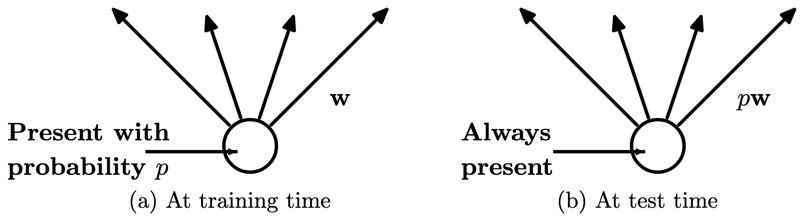
\includegraphics[width=0.6\textwidth, height=0.1\textheight, keepaspectratio]{pic/Dropout_1}
    \caption{左：训练时以概率$p$存在的单元，通过权重$\boldsymbol{w}$与下一层单元连接；右：测试时，该单元始终存在，权重 $\boldsymbol{w}$乘以$p$。测试时的输出与训练时的期望输出相同。}
    \label{fig:dropout}
\end{figure}
对于任意层$l$，$\boldsymbol{r}^{(l)}$是一个独立的随机向量，其每个元素$r_j^{(l)}$服从参数为$p$的伯努利分布。需说明的是，此处 $p$ 为神经元的\textbf{保留}概率（与原始 Dropout 论文一致，测试期对权重乘以 $p$）；而 PyTorch 的 \texttt{nn.Dropout} 及本文配置中的 $\texttt{DROPOUT\_RATE}=0.1$ 指\textbf{丢弃}概率（即 $1-p=0.1$，保留 $90\%$ 的神经元），并采用反向（inverted）Dropout——训练期对保留单元按 $1/(1-0.1)$ 放大、测试期不再缩放，二者在期望意义上等价。
向量经采样后与当前层的输出$\boldsymbol{y}^{(l)}$逐元素相乘，得到$\tilde{\boldsymbol{y}}^{(l)}$，其作为下一层的输入。
该过程在每一层均被应用，其本质是从大型网络中采样出一个子网络。

在学习阶段，损失函数的导数通过该子网络进行反向传播。测试阶段则按图\ref{fig:dropout}所示对权重进行缩放：此时神经网络以无丢弃方式运行。
\begin{figure}[H]
    \centering
    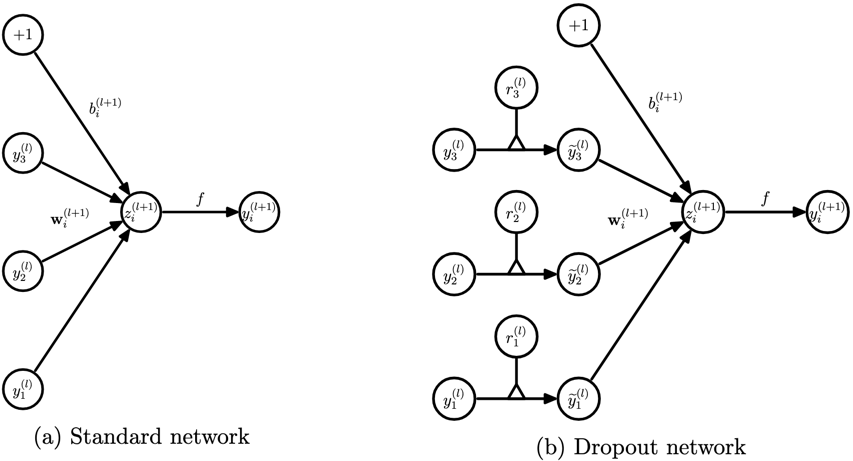
\includegraphics[width=0.8\textwidth, height=0.2\textheight, keepaspectratio]{pic/Dropout}
    \caption{标准神经网络与添加Dropout的神经网络对比图}
\end{figure}

在正向传播与权重更新过程中，标准 Dropout 以概率 $p$ 保留各神经元（即以概率 $1-p$ 暂时性地丢弃其输出及对应的连接）。
这一机制使得神经网络在每次训练迭代中都可视为一个由原网络随机采样而成的子网络，等效于在相同数据上训练大量结构略有差异的模型。

由于所有子网络共享参数并共同优化同一损失函数，最终的模型效果等价于对这些子网络预测结果的平均，从而提升了模型的稳定性与鲁棒性。
此外，Dropout 通过打破神经元之间的强依赖关系（即耦合），有效缓解了过拟合问题，增强了模型的泛化能力，显著改善了整体性能。

Dropout 在本文 ViT 模型中的应用主要体现在以下两个方面：
\begin{enumerate}[label={（\arabic*）}, leftmargin=2em, labelsep=0.5em, itemsep=0pt]
    \item 编码器中的Dropout：
    \begin{enumerate}[label={（\alph*）}, leftmargin=2em, labelsep=0.5em, itemsep=0pt]
        \item 多头注意力层中：Dropout 应用于注意力机制中 softmax 输出后的注意力权重，旨在在训练过程中以一定概率随机屏蔽部分注意力路径，从而降低模型对特定位置关系的依赖。该机制有助于抑制过拟合，提升注意力分配的鲁棒性与模型的泛化能力。
        \item 多层感知机中：Dropout 被引入至 MLP 模块中每一全连接层之后，用于在训练阶段随机丢弃部分神经元的激活输出，相当于在多个子网络之间进行模型集成。该策略有效缓解了神经元之间的共适应问题，增强了模型的正则化能力，从而提高了在未见样本上的表现。
    \end{enumerate}

    \item 解码器中的Dropout：
    \begin{enumerate}[label={（\alph*）}, leftmargin=2em, labelsep=0.5em, itemsep=0pt]
        \item 自注意力与交叉注意力层中：Dropout 同样作用于多头注意力模块中的注意力权重，分别用于解码器中处理已生成序列（自注意力）以及编码器-解码器之间的上下文建模（交叉注意力）。该机制有助于抑制注意力机制中路径依赖性过强的问题，提升模型对序列历史与图像特征之间关系的建模鲁棒性。
        \item 前馈网络中：Dropout 被用于前馈神经网络（FeedForward）模块的输出层，有效扰动神经元激活响应，降低模型在训练过程中过度拟合训练数据的风险，从而增强生成器的泛化能力。
    \end{enumerate}
\end{enumerate}

\subsubsection{早停机制}
早停机制（Early Stopping）是一种常用的正则化策略，广泛应用于深度学习模型训练过程中，旨在通过动态监控验证集上的性能表现，防止模型在训练后期出现过拟合现象。
该机制的基本思想是在模型性能不再显著提升时，自动终止训练过程，以获取最优泛化能力。其主要流程如下：
\begin{enumerate}[label={（\arabic*）}, leftmargin=2em, labelsep=0.5em, itemsep=0pt]
\item 性能监控：指定验证损失或其他评估指标作为监控对象，训练过程中持续记录模型在验证集上的性能；
\item 容忍机制：设定耐心参数（patience），允许模型在若干训练轮内性能指标未显著改善；若超过该轮数仍无改进，则认为模型已达到最优状态；
\item 权重回退：可选地在训练终止后恢复性能最优轮次对应的模型参数，以确保最终模型的泛化性能最强；
\item 资源优化：通过跳过冗余的训练轮次，能有效减少资源浪费，提升训练效率。
\end{enumerate}
综上所述，早停机制通过对模型训练过程的动态干预，实现了训练时间与模型性能之间的平衡，是提升深度学习模型泛化能力的重要技术手段之一。
  \newpage\section{模型构建}
本研究构建了一个基于 Vision Transformer（ViT）编码器与 Transformer 解码器的端到端模型框架，旨在实现数学表达式图像（涵盖印刷体与手写体）的识别与 LaTeX 转换。

其中，ViT 编码器通过自注意力机制将图像处理任务转化为序列处理任务，对输入图像进行全局建模，深入挖掘符号的空间关系与语义特征，提升对复杂结构的感知能力；Transformer 解码器则基于自注意力和交叉注意力机制，分别建模生成序列的内部依赖和编码图像与解码序列之间的对齐，从而实现对 LaTeX 序列的高质量生成。

该框架将视觉特征提取与序列生成统一于端到端结构中，便于对图像编码与 LaTeX 解码两个阶段进行联合优化。
\subsection{数据来源与预处理}
\subsubsection{数据来源}
本研究以数学表达式的结构识别与 LaTeX 转换为目标任务。考虑到方法验证需要结构清晰、标注规范且被广泛用作基准的数据集，本文选用印刷体数学表达式数据集 \texttt{im2latex-100k}\supercite{kanervisto_2016_56198} 作为主要训练与评估数据集：该数据集格式规范、规模充足，便于与现有方法进行横向对比，也便于将性能差异归因于模型本身而非数据噪声。

针对手写数学表达式这一目标应用场景，本文进一步选用手写体数据集 \texttt{MathWriting-human}\supercite{gervaisMathWritingDatasetHandwritten2025} 开展对比实验。该数据集收集了大量真实用户手写的数学表达式图像，具有较高的结构复杂性和风格多样性，更贴近实际应用场景。本文以与印刷体实验完全相同的模型架构与训练配方在该数据集上训练和评估，以考察方法向手写场景迁移的能力（见“结果与评价”一章的手写场景对比实验）。

如图~\ref{fig:dataset-samples} 所示，其中（a）（b）分别展示了手写体与印刷体数据集中具有代表性的样本图像。

\begin{figure}[H]
    \centering
    \begin{subfigure}[b]{0.48\textwidth}
        \centering
        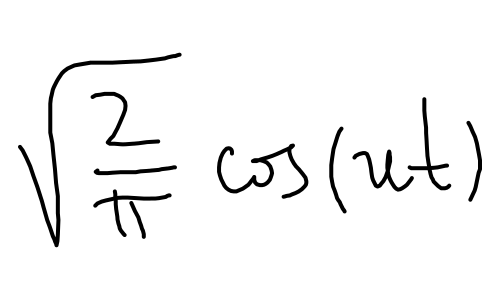
\includegraphics[width=0.9\linewidth, keepaspectratio]{pic/mathwriting-human-sample}
        \caption{\texttt{MathWriting-human} 手写体样本}
        \label{fig:mathwriting-human-sample}
    \end{subfigure}
    \hfill
    \begin{subfigure}[b]{0.48\textwidth}
        \centering
        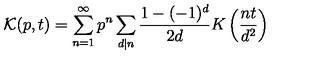
\includegraphics[width=0.9\linewidth, keepaspectratio]{pic/printed-math-expression}
        \caption{\texttt{im2latex-100k} 印刷体样本}
        \label{fig:printed-math-expression}
    \end{subfigure}
    \caption{两类数据集的代表性样本图像}
    \label{fig:dataset-samples}
\end{figure}

两个数据集的加载方式如下：
\begin{itemize}
    \item \texttt{MathWriting-human} 可通过 HuggingFace 平台获取\footnotemark[1]；
    \item \texttt{im2latex-100k} 可通过 HuggingFace 平台获取\footnotemark[2]。
\end{itemize}

\footnotetext[1]{\url{https://huggingface.co/datasets/deepcopy/MathWriting-human}；也可使用\texttt{datasets} 库命令 \texttt{load\_dataset("deepcopy/MathWriting-human")} 加载。}
\footnotetext[2]{\url{https://huggingface.co/datasets/yuntian-deng/im2latex-100k}；也可使用\texttt{datasets} 库命令 \texttt{load\_dataset("yuntian-deng/im2latex-100k")} 加载。}

本节余下内容基于 \texttt{im2latex-100k} 数据集详细介绍模型构建的完整流程。模型与数据处理流程基于 PyTorch 框架实现；该流程同样适用于 \texttt{MathWriting-human} 数据集，仅需根据具体情况对部分参数进行适当调整。下文以 $B$ 记批大小（本文实验中 $B=768$）。
\subsubsection{数据预处理}
本文对所采用的数学表达式数据集中的图像与文本数据均进行了标准化预处理操作，以提升模型训练效果与表达一致性。

图像处理主要包括尺寸规范化与像素归一化，文本处理则将 LaTeX 表达式转化为模型可读的标记序列。具体步骤如下所示：

\begin{enumerate}[label={（\arabic*）}, leftmargin=2em, labelsep=0.5em, itemsep=0pt]
\item 图像预处理：
\begin{enumerate}[label={（\alph*）}, leftmargin=2em, labelsep=0.5em, itemsep=0pt]
\item 通过 \texttt{datasets} 库载入训练数据，直接获取 PIL 格式的原始图像（RGB、尺寸不一）；
\item 将图像转换为灰度格式，通道数为 $1$；
\item 将图像统一缩放至尺寸 $50 \times 200$，并归一化像素值至 $[0,1]$ 区间；
\item 构建通道在前的图像批次张量（形状 $[B, 1, 50, 200]$），满足模型输入维度要求；
\end{enumerate}
\item 文本预处理：
\begin{enumerate}[label={（\alph*）}, leftmargin=2em, labelsep=0.5em, itemsep=0pt]
\item 载入训练数据，为每条 LaTeX 表达式添加特殊标记 \texttt{[START]} 与 \texttt{[END]}；
\item 词元规范化：\texttt{im2latex-100k} 的公式已是空格分隔的词元序列，直接按空白切分；\texttt{MathWriting-human} 的 \texttt{latex} 字段为未分词的原始字符串（如 \texttt{V(\textbackslash tilde\{\textbackslash beta\})}），先以正则规则切分为词元——LaTeX 命令（含星号形式，如 \texttt{\textbackslash operatorname*}）、转义符号（如 \texttt{\textbackslash\%}）各为一个词元，其余按单字符切分（数字逐位拆分，与 \texttt{im2latex} 约定一致）——再以空格连接，统一两个数据集的词元约定；
\item 构建基于训练语料的分词器（Tokenizer）：按空白切分词元、保留大小写与全部 LaTeX 符号，词表按词频降序构建并约定索引 $0$ 为填充符、索引 $1$ 为 \texttt{[UNK]}，确保转换过程中保留语义及语法信息；
\item 使用分词器将 LaTeX 表达式转换为整数索引序列，并后向填充至固定长度 $152$；
\end{enumerate}
\end{enumerate}
\subsection{编码器：Vision Transformer}
本文引入 Vision Transformer（ViT）作为编码器，以增强模型对手写数学表达式图像中复杂结构与全局语义的建模能力。
ViT 首先将输入图像划分为固定大小的图像块（patch），再将每个图像块展平并嵌入高维特征空间，构建图像块序列以供 Transformer 编码器处理。
得益于全局自注意力机制，ViT 能直接建模图像中远距离符号之间的依赖关系，不受卷积网络局部感受野的约束。

相比基于 CNN 的方法，ViT 在建模长程结构依赖方面更具优势，适用于结构复杂、符号排列多变的数学表达式图像。
其对图像空间结构的建模能力为解码器生成 LaTeX 序列提供了图像特征表示（生成质量见“结果与评价”一章）。

\subsubsection{序列化处理}
\begin{enumerate}[label={（\arabic*）}, leftmargin=2em, labelsep=0.5em, itemsep=0pt]
    \item 图像分块：将输入图像（$\texttt{IMG\_SHAPE}=[50, 200, 1]$）划分为 $\texttt{PATCH\_SIZE}=10 \times 10$ 的非重叠图像块，得到 $\texttt{NUM\_PATCHES}=(50 \div 10) \times (200 \div 10) = 100$ 个图像块，并重组为序列形式；
    \item 线性投影：将 $\texttt{NUM\_PATCHES}=100$ 个图像块组成的序列输入线性层，映射至维度为 $\texttt{EMBEDDING\_DIM}=256$ 的特征空间，获取图像块的高维表示；
    \item 位置编码：为每个图像块分配可学习的位置编码，采用 $[0, \cdots, \texttt{NUM\_PATCHES}-1]=[0, 1, \cdots, 99]$ 作为索引，以建模图像块在原图中的空间位置信息；
    \item 输入序列构建：将图像块特征与对应位置编码逐元素相加，组成输入序列，形状为 $[B, \texttt{NUM\_PATCHES}, \texttt{EMBEDDING\_DIM}] = [B, 100, 256]$，作为 Transformer 编码器的输入。
\end{enumerate}
注：如“Vision Transformer 基本原理”一章所述，序列生成任务使用编码器输出的全部图像块特征序列，而非面向分类的 [CLS] 全局表征。因此本文不引入“可学习类别标记”：编码器直接输出与 $100$ 个图像块一一对应的特征序列，作为解码器交叉注意力的键与值，由其完成视觉—文本对齐。该设计与目标任务的序列生成性质一致，同时避免了 [CLS] 标记引入的额外位置与计算开销。
\subsubsection{编码器架构}
\begin{enumerate}[label={（\arabic*）}, leftmargin=2em, labelsep=0.5em, itemsep=0pt]
    \item 层归一化：参数$\epsilon=10^{-6}$（代码中 \texttt{epsilon=1e-6}），对输入序列进行归一化处理，确保数值稳定性；
    \item 多头自注意力：采用 $\texttt{NUM\_HEADS}=4$ 个头的多头自注意力机制（\texttt{nn.MultiheadAttention}），总嵌入维度 $\texttt{EMBEDDING\_DIM}=256$ 平均分配至各头，每头维度为 $256 \div 4 = 64$；注意力权重的 Dropout 概率为 $\texttt{DROPOUT\_RATE}=0.1$；
    \item 残差连接：将多头自注意力的输出与输入序列相加，形成残差连接，增强梯度流动；
    \item 层归一化：参数$\epsilon=10^{-6}$（代码中 \texttt{epsilon=1e-6}），对残差连接进行归一化处理，确保数值稳定性；
    \item 多层感知机（MLP）：由两个线性层构成（$256 \to 512 \to 256$），每个线性层之后均接 GELU 激活与 Dropout（概率 $\texttt{DROPOUT\_RATE}=0.1$），整体呈扩展—收缩结构，其中：
    \begin{itemize}
        \item 扩展阶段：线性层 $\texttt{nn.Linear(256, 512)}$ 将特征由 $\texttt{EMBEDDING\_DIM}=256$ 维升至 $512$ 维，随后经 GELU 激活与 Dropout，以增强非线性表达能力（GELU 相比 ReLU 梯度更平滑，有利于训练稳定）；
        \item 收缩阶段：线性层 $\texttt{nn.Linear(512, 256)}$ 将特征降回 $\texttt{EMBEDDING\_DIM}=256$ 维，同样经 GELU 激活与 Dropout，使输出维度与输入一致，便于残差连接；
        \item 设计原理：扩展-收缩模式遵循标准Transformer架构，通过先扩展后收缩的方式，在保持输入输出维度匹配的同时，增强非线性表达能力。
    \end{itemize}
    \item 残差连接：将 MLP 输出与第一个残差连接的输出相加，形成第二个残差连接，进一步增强梯度流动；
\end{enumerate}
将上述结构重复 $\texttt{TRANSFORMER\_LAYERS}=8$ 次，形成深度Transformer编码器，增强模型的表达能力。
随后对最后一个Transformer块的输出进行最终层归一化处理（$\texttt{epsilon=1e-6}$），确保特征表示的数值稳定性。
最终输出：经过 $8$ 层Transformer块处理和最终归一化后的特征表示，形状为 $[B, \texttt{NUM\_PATCHES}, \texttt{EMBEDDING\_DIM}]=[B, 100, 256]$，其中 $\texttt{NUM\_PATCHES}=(50 \div 10) \times (200 \div 10) = 100$。

\subsection{解码器：Transformer}
本文采用标准的 Transformer 解码器结构，将编码器提取的图像表示自回归地映射为结构化的 LaTeX 序列。该解码器融合自注意力与交叉注意力机制，协同建模目标序列的内部依赖与图像特征之间的对应关系。

其中，交叉注意力机制通过引导解码器聚焦于编码器输出中与当前生成阶段最相关的图像区域特征，提升视觉-语言对齐效果；
而自注意力机制则用于捕捉目标序列内部的依赖关系，确保解码过程中的上下文一致性与语义连贯性。
该双重注意力结构旨在同时建模目标序列的内部依赖与图像—文本对齐关系，为高质量的 LaTeX 序列生成提供结构支撑（实际效果见“结果与评价”一章）。

\subsubsection{解码器架构}
\begin{enumerate}[label={（\arabic*）}, leftmargin=2em, labelsep=0.5em, itemsep=0pt]
    \item 序列嵌入层（SeqEmbedding）：
        \begin{enumerate}[label={（\alph*）}, leftmargin=2em, labelsep=0.5em, itemsep=0pt]
            \item 词元嵌入：将输入的词元 ID转换为向量表示，维度为$\texttt{EMBEDDING\_DIM}=256$，并与可学习的位置编码逐元素相加融合；
            \item 填充处理：嵌入层指定 $\texttt{padding\_idx}=0$，将填充符的嵌入向量固定为零且不参与梯度更新；填充位置对优化目标的影响则由掩蔽损失函数（见“训练原理”一章）予以排除；
            \item 位置编码采用可学习的嵌入方式（$\texttt{nn.Embedding(max\_length, depth)}$），最大序列长度为$\texttt{MAX\_SEQ\_LEN\_1}=151$；为防止位置索引越界，解码前对输入序列统一截断至该长度。
        \end{enumerate}
    \item 因果自注意力层（CausalSelfAttention）：
        \begin{enumerate}[label={（\alph*）}, leftmargin=2em, labelsep=0.5em, itemsep=0pt]
            \item 输入为解码器当前的嵌入序列，设动态序列长度为\texttt{seq\_length}，则其形状为$[B, \texttt{seq\_length}, \texttt{EMBEDDING\_DIM}] = [B, \texttt{seq\_length}, 256]$：
                \begin{itemize}
                    \item 训练阶段：教师强制下取 $\texttt{sequences[:, :-1]}$ 作为输入，$\texttt{seq\_length}$ 固定为 $\texttt{MAX\_SEQ\_LEN\_1}=151$，填充位置由掩蔽损失从优化目标中排除；
                    \item 推理阶段：$\texttt{seq\_length}$ 从 $1$（仅含 $\texttt{[START]}$）开始，随自回归生成逐词元增长，直至生成 $\texttt{[END]}$ 或达到 $\texttt{MAX\_SEQ\_LEN\_1}=151$。
                \end{itemize}
            \item 使用因果掩码：构造上三角布尔矩阵作为注意力掩码（$\texttt{torch.triu}$，对角线以上为屏蔽位置），确保解码器只能查看到已经生成的部分，并避免信息泄漏；
            \item 使用残差连接和层归一化（本文解码器采用 Post-LN，即先残差相加再归一化 $\text{LayerNorm}(\boldsymbol{x}+\text{Sublayer}(\boldsymbol{x}))$，与编码器的 Pre-LN 相对），增强梯度流动和训练稳定性；
            \item 采用 $\texttt{DECODER\_HEADS}=8$ 头的多头注意力机制，总嵌入维度 $256$ 平均分配至各头，每头维度为 $256 \div 8 = 32$。
        \end{enumerate}
    \item 交叉注意力层（CrossAttention）：
\begin{enumerate}[label={（\alph*）}, leftmargin=2em, labelsep=0.5em, itemsep=0pt]
    \item 查询为文本序列，键与值为图像特征序列，输出为融合了图像信息的文本隐藏表示（并非最终 LaTeX 序列，后者还需经前馈层与输出层进一步生成）；
    \item 图像特征形状为$[B, \texttt{NUM\_PATCHES}, \texttt{EMBEDDING\_DIM}] = [B, 100, 256]$（基于$\texttt{IMG\_SHAPE}=[50, 200, 1]$图像和$\texttt{PATCH\_SIZE}=10 \times 10$的图像块大小），文本序列形状为$[B, \texttt{seq\_length}, 256]$，其中：
    \begin{itemize}
        \item 图像特征：来自ViT编码器的输出，包含$100$个图像块的特征表示，每个图像块对应图像中的一个$10 \times 10$区域；
        \item 文本序列：来自解码器的当前嵌入状态，长度$\texttt{seq\_length}$为动态值；
        \item 跨模态融合：以文本序列为查询（Query）、图像特征为键与值（Key/Value）调用多头注意力（$\texttt{mha(x, y, y)}$），实现文本对图像特征的注意力机制。
    \end{itemize}
    \item 使用残差连接与层归一化；并保存交叉注意力分数（形状 $[B, \texttt{seq\_length}, \texttt{NUM\_PATCHES}]$，各头取平均）用于可视化，以分析生成各词元时模型关注的图像区域。
\end{enumerate}
\item 前馈网络层（FeedForward）：
\begin{enumerate}[label={（\alph*）}, leftmargin=2em, labelsep=0.5em, itemsep=0pt]
    \item 由两个线性层构成（单个隐藏层，维度 $\texttt{EMBEDDING\_DIM} \times 2 = 512$；输出维度回到 $\texttt{EMBEDDING\_DIM} = 256$），采用扩展-收缩结构，其中：
    \begin{itemize}
        \item 第一层：$\texttt{nn.Linear(256, 512)}$，使用ReLU激活函数，将输入特征从256维扩展至512维，增强模型的非线性表达能力；
        \item 第二层：$\texttt{nn.Linear(512, 256)}$，无激活函数（线性激活），将特征维度收缩回256维，保持与输入维度一致，便于残差连接；
        \item Dropout层：概率为$\texttt{DROPOUT\_RATE}=0.1$，在训练时随机丢弃部分神经元激活，防止过拟合并增强模型泛化能力。
    \end{itemize}
\end{enumerate}
    \item 解码器层（DecoderLayer）：
        \begin{enumerate}[label={（\alph*）}, leftmargin=2em, labelsep=0.5em, itemsep=0pt]
            \item 共三个子层：因果自注意力层、交叉注意力层和前馈网络层，其中两个注意力子层均采用 $\texttt{DECODER\_HEADS}=8$ 头的多头注意力机制，其中：
            \begin{itemize}
                \item 因果自注意力：处理文本序列内部依赖关系，使用上三角因果掩码确保每个位置只能访问之前的位置，防止信息泄漏；
                \item 交叉注意力：实现文本对图像特征的注意力机制，其中文本序列作为查询、图像特征作为键值对，实现跨模态信息融合；
                \item 前馈网络：进行非线性特征变换，采用扩展-收缩结构增强模型表达能力。
            \end{itemize}
            \item 层内数据流为 $\texttt{out\_seq} \rightarrow \texttt{self\_attention} \rightarrow \texttt{cross\_attention} \rightarrow \texttt{ff} \rightarrow \texttt{output}$；输入为图像特征 $[B, 100, 256]$ 与文本嵌入 $[B, \texttt{seq\_length}, 256]$，输出为跨模态融合后的文本表示。
            \item 多层堆叠设计的原因和优势：本文将上述解码器层堆叠 $\texttt{DECODER\_LAYERS}=4$ 层，其考量如下：
            \begin{itemize}
                \item 表达能力：逐层细化对目标序列内部依赖与跨模态对齐的建模，相比单层结构能够刻画更深层次的层次结构与语法关系，提升 LaTeX 序列生成质量；
                \item 计算复杂度：自注意力的计算复杂度为 $O(\texttt{DECODER\_LAYERS} \times n^2 \times d)$，其中 $n$ 为序列长度、$d$ 为特征维度（此处略去同阶的交叉注意力开销）；在 $\texttt{MAX\_SEQ\_LEN\_1}=151$ 的最大序列长度下，$4$ 层堆叠的计算与显存开销仍处于可接受范围；
                \item 多头建模：每层均采用 $\texttt{DECODER\_HEADS}=8$ 头的多头注意力，使模型能够在多个表示子空间中并行建模不同范围的依赖关系；
                \item 训练稳定性：每个子层均配合残差连接与层归一化，有效缓解深层堆叠下的梯度消失与爆炸风险，保证多层结构的训练稳定性。
            \end{itemize}
        \end{enumerate}
    \item Token输出层（TokenOutput）：
        \begin{enumerate}[label={（\alph*）}, leftmargin=2em, labelsep=0.5em, itemsep=0pt]
            \item 通过线性层 $\texttt{nn.Linear(256, vocab\_size)}$ 将解码器特征（$[B, \texttt{seq\_length}, 256]$）映射到词汇表维度（$[B, \texttt{seq\_length}, \texttt{vocab\_size}]$），词汇表大小由分词器动态确定；
            \item 集成偏置调整机制，根据训练数据统计信息调整词元生成概率，禁止生成空字符串和未知词元（$\texttt{banned\_tokens}=('', '[UNK]')$），其中：
            \begin{itemize}
                \item 统计计算：以 $\texttt{torch.bincount}$ 统计训练标签中每个词元的出现频率，构建词元频率分布；
                \item 概率计算：将频率归一化为概率分布 $p$，并取对数得到先验偏置 $\log p$；
                \item 禁止机制：将未在训练数据中出现的词元（含被禁词元）的偏置设为 $-10^9$，在后续 Softmax（损失计算或采样）中使其概率接近零；
                \item 持久化：偏置注册为模型缓冲区（buffer），随权重一同保存与加载，保证推理时无需重新统计。
            \end{itemize}
            \item 输出为未归一化的 logits（形状 $[B, \texttt{seq\_length}, \texttt{vocab\_size}]$，不再施加 Softmax）：在线性映射结果上加对数先验偏置后直接返回，以与损失函数 $\texttt{F.cross\_entropy}$ 及推理阶段的 $\texttt{argmax}$／温度采样（均以 logits 为输入）保持一致，避免重复施加 Softmax。
            \item 通过$\texttt{adapt()}$方法根据训练数据调整输出层的偏置项，优化生成质量，计算信息熵以评估词汇表分布，其中：
            \begin{itemize}
                \item 信息熵计算：$\texttt{entropy = -(log\_p*p).sum()}$，即词元边际分布的香农熵，用以刻画其相对均匀分布的集中程度（熵越大越接近均匀，越小表示词频越集中）；
                \item 对比分析：输出均匀熵（$\ln(\texttt{vocab\_size})$）和边际熵，评估词汇表的使用效率（本文词表二者分别为 $6.22$ 与 $3.83$）；
                \item 质量优化：通过偏置调整，使模型更倾向于生成训练数据中常见的词元，提高生成文本的质量和合理性；
                \item 训练适配：$\texttt{adapt()}$方法在训练前调用，确保偏置项与训练数据分布一致。
            \end{itemize}
        \end{enumerate}
    \item 完整Captioner模型：
        \begin{enumerate}[label={（\alph*）}, leftmargin=2em, labelsep=0.5em, itemsep=0pt]
            \item 集成ViT编码器（$\texttt{feature\_extractor}$）和Transformer解码器，实现端到端的图像到文本生成，其中：
            \begin{itemize}
                \item 特征提取：将输入图像（形状为$[B, 1, 50, 200]$）转换为特征表示（形状为$[B, 100, 256]$），通过ViT编码器提取图像的语义特征；
                \item 文本处理：通过分词器将输入文本转换为词元序列，并截断至位置嵌入支持的最大长度；
                \item 序列嵌入：将词元序列转换为嵌入表示（形状为$[B, \texttt{seq\_length}, 256]$），包含词元嵌入和位置编码的融合。
            \end{itemize}
            \item 支持自回归文本生成，采用温度控制策略（$\texttt{temperature}=0$为贪婪解码，$>0$为采样解码），其中：
            \begin{itemize}
                \item 贪婪解码：选择 logits 最大的词元（$\texttt{argmax}$），确保生成结果的确定性和一致性；
                \item 采样解码：将 logits 除以温度参数后施加 Softmax 得到分布，再按多项式分布采样（$\texttt{torch.multinomial}$），温度越大随机性越强；
                \item 预测 logits：取最后一个时间步的未归一化预测得分，形状为$[1, \texttt{vocab\_size}]$。
            \end{itemize}
            \item 使用特殊标记$\texttt{[START]}$和$\texttt{[END]}$控制生成过程，最大生成长度为$\texttt{MAX\_SEQ\_LEN\_1}=151$，其中：
            \begin{itemize}
                \item 起始标记：$\texttt{[START]}$用于标识生成序列的开始，经分词器转换为词元 ID 后作为初始输入；
                \item 结束标记：$\texttt{[END]}$用于标识生成序列的结束，当检测到该标记时停止生成过程；
                \item 长度控制：以最大生成长度作为循环上界，防止无限生成。
            \end{itemize}
            \item 提供 $\texttt{simple\_gen()}$ 方法实现自回归（贪婪／温度采样）解码，逐词元生成 LaTeX 序列并支持生成过程可视化，其中：
            \begin{itemize}
                \item 初始标记：设置生成起始标记，形状为$[1, 1]$，包含起始词元 ID；
                \item 序列扩展：将新生成的词元拼接到当前序列末尾，实现序列的逐步增长；
                \item 结束检测：检测生成结束条件，当生成结束标记时跳出循环；
                \item 结果转换：将词元 ID序列转换回可读文本：先去除起始标记，仅当序列确实以$\texttt{[END]}$结尾时才去除末位词元，避免在达到最大长度仍未生成$\texttt{[END]}$时误删最后一个有效词元；
                \item 文本拼接：将词元序列以空格连接为完整的 LaTeX 字符串；
                \item 推理模式：生成全程在 $\texttt{torch.no\_grad()}$ 与评估模式（关闭 Dropout）下进行，结束后恢复原训练状态。
            \end{itemize}
            \item 模型架构的核心组件和设计特点：
            \begin{itemize}
                \item 双向映射：分词器提供词元与 ID之间的双向转换，支持词汇表的动态构建；
                \item 多层解码：由多个相同的 Transformer 解码器层堆叠而成，每层包含因果自注意力、交叉注意力与前馈网络，实现深度特征融合；
                \item 端到端训练：整个模型支持端到端训练，采用自定义训练循环进行批量训练，损失函数为掩蔽交叉熵损失（$\texttt{masked\_loss}$，基于 logits 计算并忽略 padding 位置）；
                \item 灵活推理：支持单张图像推理和批量推理，提供贪婪/温度采样（$\texttt{simple\_gen()}$）与束搜索（$\texttt{beam\_gen()}$）两类生成接口。
            \end{itemize}
        \end{enumerate}
\end{enumerate}

\subsection{模型训练与推理}
\subsubsection{训练策略}
\begin{enumerate}[label={（\arabic*）}, leftmargin=2em, labelsep=0.5em, itemsep=0pt]
    \item 优化器配置：采用 AdamW 优化器（将权重衰减与梯度更新解耦，$\beta_1=0.9$、$\beta_2=0.98$、$\epsilon=10^{-9}$），权重衰减系数为 $0.0001$；学习率采用 Transformer 原论文的预热调度策略\supercite{vaswaniAttentionAllYou2017}：
    \begin{equation}
        lr(t) = d_{\text{model}}^{-0.5} \cdot \min\left(t^{-0.5},\ t \cdot t_{\text{warmup}}^{-1.5}\right),
    \end{equation}
    其中 $d_{\text{model}}=\texttt{EMBEDDING\_DIM}=256$，$t_{\text{warmup}}=\texttt{WARMUP\_STEPS}=800$：前 $800$ 步学习率线性升温（峰值约 $2.2\times10^{-3}$），此后按 $1/\sqrt{t}$ 衰减；预热步数依据批大小（$768$，每轮约 $52$ 个优化步）设定——$800$ 步约对应第 $15$ 轮、占早停时总优化步数（约 $4{,}100$ 步）的 $1/5$；
    \item 梯度裁剪：每次反向传播后、参数更新前对梯度施加全局范数裁剪（阈值 $1.0$），防止预热峰值学习率附近的异常梯度引发训练发散（原理见“训练原理”一章，实验证据见“结果与评价”一章）；
    \item 损失函数设计：使用交叉熵损失函数，配合掩码机制处理变长序列，通过忽略填充词元（padding token）的影响，确保损失计算仅基于有效词元，提升训练效率；
    \item 训练参数设置：批次大小设置为 $768$，最大训练轮数为 $100$，验证集划分比例为 20\%：以固定随机种子（$42$）对训练数据随机划分，避免数据集内部排序导致的验证集分布偏置，并保证划分可复现；
    \item 正则化策略：在编码器和解码器中均采用Dropout正则化（概率为 $0.1$），结合权重衰减（weight decay）防止过拟合，同时实现早停机制（patience=10）和最优权重检查点保存（监控验证损失，训练结束自动回退至最优轮次权重）。
\end{enumerate}

\subsubsection{推理机制}
\begin{enumerate}[label={（\arabic*）}, leftmargin=2em, labelsep=0.5em, itemsep=0pt]
    \item 自回归生成策略：采用逐词元生成机制，每个时间步基于已生成序列$y_{<t}$和图像特征$f(I)$预测下一个词元 $y_t$，通过因果自注意力机制确保生成过程的因果性约束；
    \item 解码策略：支持三种生成策略：贪婪解码（temperature=0）选择概率最高的词元；随机采样（temperature>0）通过温度参数调节概率分布的尖锐程度，平衡生成文本的多样性与准确性；束搜索（beam search，束宽 $\texttt{BEAM\_WIDTH}=4$）按 Transformer 原论文配方\supercite{vaswaniAttentionAllYou2017}并行维护多条候选序列，并以 GNMT 长度惩罚\supercite{wuGoogleNeuralMachine2016} $lp(Y)=\left((5+|Y|)/6\right)^{\alpha}$（$\alpha=0.6$）对各候选的累计对数概率归一化后选取整体得分最高的候选序列（束搜索为近似搜索，并不保证全局最优），缓解贪婪解码的局部最优问题；
    \item 序列长度控制：通过最大序列长度限制（151个词元）和结束标记（[END]）检测机制控制生成序列长度，避免无限生成和资源浪费；
    \item 质量保证机制：通过TokenOutput层的偏置调整机制，基于训练数据中词元频率分布计算先验概率，同时禁止生成特定词元（如空字符串和[UNK]），提升生成文本的语义合理性和语法正确性。
\end{enumerate}

\subsubsection{训练监控与评估}
\begin{enumerate}[label={（\arabic*）}, leftmargin=2em, labelsep=0.5em, itemsep=0pt]
    \item 训练监控：实时监控训练和验证的损失及准确率，并在每个epoch结束后对固定样本图像生成示例文本，直观评估模型训练进展；
    \item 模型保存策略：采用最佳权重保存机制，基于验证损失监控模型性能，自动保存验证损失最小的模型权重，确保获得最优模型状态；
    \item 性能评估指标：除基础准确率外，支持BLEU-4分数计算、可视化预测结果展示，以及交互式文本生成演示，全面评估模型在图像描述生成任务上的表现。
\end{enumerate}
  \newpage\section{结果与评价}
\subsection{实验设置}
\subsubsection{实验环境与数据划分}
本文全部实验在单张 NVIDIA GeForce RTX 5090（32 GB 显存）上完成，软件环境为 Linux 操作系统、Python 3.11 与 PyTorch 2.12（CUDA 13.0）。

实验数据取自 \texttt{im2latex-100k} 数据集：从其训练划分中选取 $50{,}000$ 个样本，
并以固定随机种子（$\texttt{SPLIT\_SEED}=42$）随机划分为 $40{,}000$ 个训练样本与 $10{,}000$ 个验证样本；
测试集取自该数据集独立的测试划分，共 $2{,}000$ 个样本。
采用固定种子的随机划分而非按顺序截取末尾样本，是为了避免数据集内部可能存在的排序偏置
（如按公式长度排序）导致验证集分布失真，同时保证数据划分可复现（训练过程的权重初始化、Dropout 与批次打乱未设全局种子，不同次训练的结果未必逐位一致，参见后文训练稳定性分析）。
基于训练语料构建的词表共含 $504$ 个词元（含填充符与 \texttt{[UNK]}），
其边际熵为 $3.83$，显著低于均匀分布熵 $\ln 504 \approx 6.22$，
表明 LaTeX 词元分布高度不均衡，这也是输出层引入词频先验偏置的依据。

\subsubsection{超参数配置}
模型与训练的完整超参数配置如表~\ref{tab:hyperparams} 所示。
模型总参数量为 $7.73$M，其中 ViT 编码器 $4.27$M、解码器（含嵌入与输出层）$3.46$M，
属轻量级配置。

\begin{table}[htbp]
    \centering
    \caption{模型与训练超参数配置}
    \begin{tabular}{llll}
        \toprule
        \textbf{类别} & \textbf{超参数} & \textbf{取值} & \textbf{说明} \\
        \midrule
        \multirow{4}{*}{输入}
        & 图像尺寸 & $50 \times 200 \times 1$ & 灰度图，像素归一化至 $[0,1]$ \\
        & 图像块大小 & $10 \times 10$ & 共 $100$ 个图像块 \\
        & 词表大小 & $504$ & 含填充符与 \texttt{[UNK]} \\
        & 最大序列长度 & $152$ & 含 \texttt{[START]}/\texttt{[END]} \\
        \midrule
        \multirow{3}{*}{编码器}
        & 层数 / 注意力头数 & $8$ / $4$ & 每头维度 $256/4=64$ \\
        & 嵌入维度 & $256$ & — \\
        & MLP 隐藏维度 & $[512, 256]$ & GELU 激活 \\
        \midrule
        \multirow{2}{*}{解码器}
        & 层数 / 注意力头数 & $4$ / $8$ & 每头维度 $256/8=32$ \\
        & 前馈网络维度 & $512 \to 256$ & ReLU 激活 \\
        \midrule
        \multirow{6}{*}{训练}
        & 批大小 & $768$ & 每轮约 $52$ 个优化步 \\
        & 优化器 & AdamW & $\beta_1{=}0.9$，$\beta_2{=}0.98$，$\epsilon{=}10^{-9}$ \\
        & 权重衰减 & $10^{-4}$ & 解耦式权重衰减 \\
        & 学习率调度 & 预热 $800$ 步 & 峰值约 $2.2\times10^{-3}$ \\
        & 梯度裁剪 & 全局范数 $1.0$ & 防止训练发散 \\
        & Dropout / 早停 & $0.1$ / patience $10$ & 监控验证损失 \\
        \bottomrule
    \end{tabular}
    \label{tab:hyperparams}
\end{table}

\subsection{训练过程与稳定性分析}
\subsubsection{收敛过程}
图~\ref{fig:training-history} 给出了训练与验证集上掩蔽损失和掩蔽准确率随训练轮次的变化曲线。
训练在第 $78$ 轮由早停机制终止：验证损失在第 $68$ 轮达到最优值 $0.4427$（对应验证准确率 $90.5\%$），
其后连续 $10$ 轮未再改善，训练终止并自动回退至最优轮次的权重。
整个训练过程损失单调平稳下降，未出现震荡或发散；
训练与验证曲线在前 $25$ 轮几乎重合，其后训练损失继续下降而验证损失趋于平台（最终训练损失 $0.105$、验证损失约 $0.45$），
呈现轻度而可控的过拟合，早停机制有效阻止了其进一步扩大。

\begin{figure}[H]
    \centering
    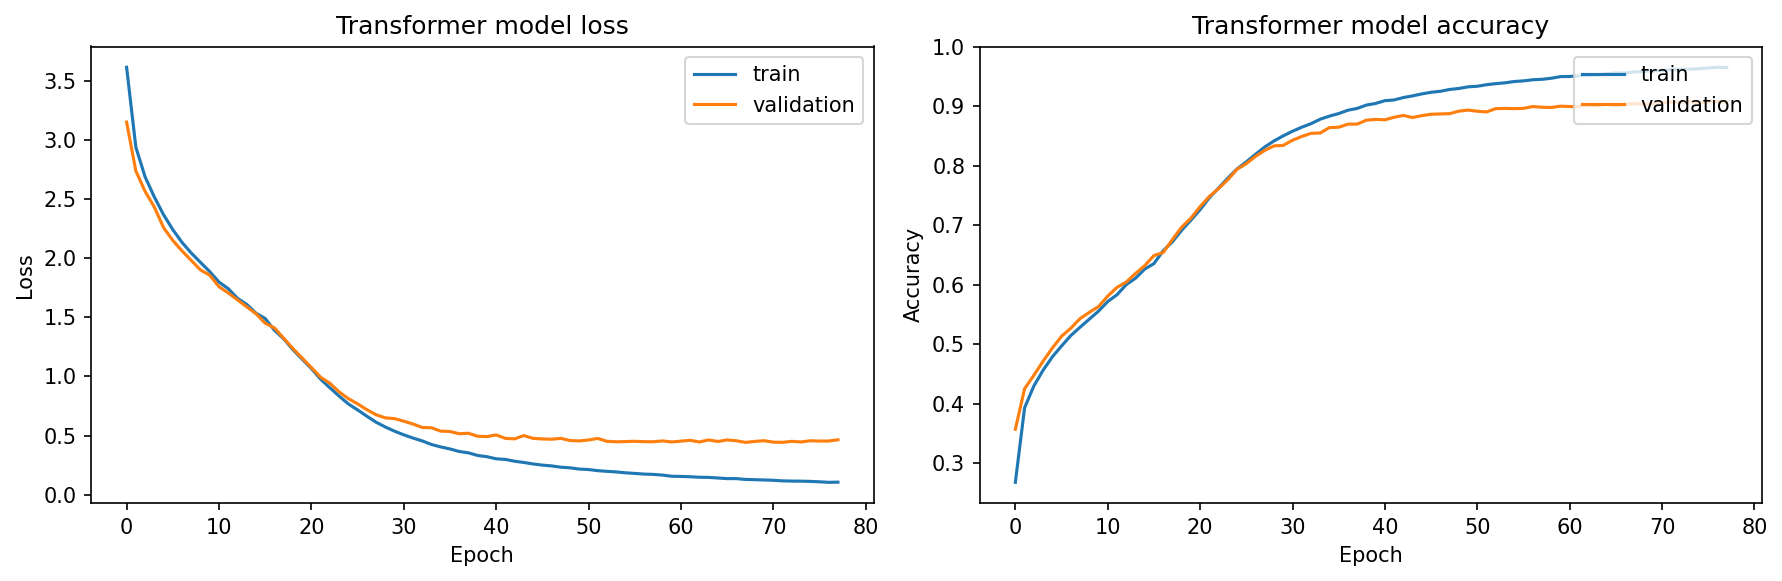
\includegraphics[width=\textwidth]{pic/training_history}
    \caption{训练与验证集上的掩蔽损失（左）与掩蔽准确率（右）变化曲线}
    \label{fig:training-history}
\end{figure}

\subsubsection{训练稳定性与梯度裁剪的必要性}
在大批量（$768$）配合预热调度的设定下，本文实验观察到了显著的训练稳定性问题，
为梯度裁剪的必要性提供了直接的实验证据：

\begin{enumerate}[label={（\arabic*）}, leftmargin=2em, labelsep=0.5em, itemsep=0pt]
    \item {无梯度裁剪时训练对随机性高度敏感}：在预热步数为 $500$（峰值学习率约 $2.8\times10^{-3}$）、
    无梯度裁剪的配置下，两次仅随机种子不同的训练呈现截然不同的结局——
    一次正常收敛，另一次在第 $7$ 轮（恰处于学习率爬升至峰值附近的阶段）突然发散：
    损失由 $2.07$ 跳升至 $4.02$，此后模型坍缩为退化解，
    无论输入何种图像均重复输出最高频词元 \texttt{\{} 与 \texttt{\}}，
    掩蔽准确率恰好卡死在该类词元的边际频率（约 $16.4\%$）附近，且无法依靠后续训练自行恢复；
    \item {发散机理}：预热阶段后期学习率接近峰值，此时单个梯度范数异常的批次即可在一步更新中
    将权重推离正常区域；模型一旦落入“仅输出高频词元”的退化局部极小，
    其梯度信号近乎平坦，以衰减后的学习率难以逃逸；
    \item {修复措施及效果}：引入全局范数为 $1.0$ 的梯度裁剪，并将预热步数提高至 $800$
    （峰值学习率降至约 $2.2\times10^{-3}$）后，训练全程（$78$ 轮、约 $4{,}100$ 个优化步）
    未再出现任何失稳迹象；在本次对比中，其最终验证损失亦略低于此前无裁剪的成功训练
    （$0.4427$ 对 $0.4628$；两次训练的预热步数不同，此处仅作参考）。
\end{enumerate}

该现象与 Transformer 训练的已有经验一致：在大批量、强预热的设定下，
梯度裁剪并非可选的保守措施，而是保证训练可靠完成的必要组件。

\subsection{主要结果}
模型在独立测试集（$2{,}000$ 个样本）上的总体性能如表~\ref{tab:results} 所示。
其中掩蔽损失与掩蔽准确率在教师强制（teacher forcing）模式下逐词元计算（按批次求均值后再对批次取平均）；
BLEU-4 分数则在完全自回归生成模式下计算（对 $500$ 个测试样本解码，
采用 method1 平滑），更真实地反映模型实际推理时的生成质量。

\begin{table}[H]
    \centering
    \caption{模型在 \texttt{im2latex-100k} 测试集上的总体性能}
    \begin{tabular}{lcc}
        \toprule
        \textbf{指标} & \textbf{评估模式} & \textbf{数值} \\
        \midrule
        掩蔽损失（Masked Loss） & 教师强制 & $0.4551$ \\
        掩蔽准确率（Masked Accuracy） & 教师强制 & $90.14\%$ \\
        BLEU-4（贪婪解码） & 自回归生成 & $0.6767$ \\
        BLEU-4（束搜索，$k=4$） & 自回归生成 & $\mathbf{0.7012}$ \\
        \bottomrule
    \end{tabular}
    \label{tab:results}
\end{table}

对上述结果作如下分析：
\begin{enumerate}[label={（\arabic*）}, leftmargin=2em, labelsep=0.5em, itemsep=0pt]
    \item {泛化一致性}：测试集掩蔽损失（$0.4551$）与验证集最优损失（$0.4427$）十分接近，
    测试准确率（$90.14\%$）与验证准确率（$90.5\%$）基本持平，
    表明模型未对验证集产生选择性过拟合，所报告的性能具有可靠的泛化意义；
    \item {教师强制指标与生成指标的差距}：教师强制下逐词元准确率达 $90.14\%$，
    而自回归生成的 BLEU-4 为 $0.68 \sim 0.70$。二者的差距源于自回归解码的误差累积效应——
    教师强制模式下每一步均以真实历史为条件，而实际生成中早期的词元错误会改变后续所有预测的条件分布。
    这一差距也印证了仅以教师强制准确率评估生成模型会系统性高估其实际能力，
    自回归 BLEU 才是更接近真实使用场景的指标；
    \item {与代表性方法的关系}：在相同数据集上，以全分辨率图像和更大模型容量为代价的专用方法
    （如基于由粗到细注意力的模型\supercite{dengImagetomarkupGenerationCoarsetofine2017}）
    报告了更强的识别性能；需说明的是，其评测协议（分词方式、平滑策略与样本规模）与本文不完全一致，相关数值不宜直接逐位比较。本文模型以 $50\times200$ 的低分辨率输入与 $7.73$M 的轻量参数规模
    取得约 $0.70$ 的 BLEU-4，在该量级的轻量配置下验证了纯 Transformer 架构在该任务上的有效性；
    分辨率与模型容量带来的性能上限将在第~\ref{subsec:limitations} 节进一步讨论。
\end{enumerate}

\subsection{解码策略对比}
为考察解码策略对生成质量的影响，在同一组 $500$ 个测试样本上分别采用贪婪解码与束搜索解码
（束宽 $k=4$，GNMT 长度惩罚\supercite{wuGoogleNeuralMachine2016} $\alpha=0.6$）\supercite{vaswaniAttentionAllYou2017}，结果如表~\ref{tab:decoding} 所示。

\begin{table}[H]
    \centering
    \caption{贪婪解码与束搜索解码的 BLEU-4 对比（同一组 500 个测试样本）}
    \begin{tabular}{lccc}
        \toprule
        \textbf{解码策略} & \textbf{BLEU-4} & \textbf{绝对提升} & \textbf{相对提升} \\
        \midrule
        贪婪解码 & $0.6767$ & — & — \\
        束搜索（$k=4$，$\alpha=0.6$） & $\mathbf{0.7012}$ & $+0.0245$ & $+3.6\%$ \\
        \bottomrule
    \end{tabular}
    \label{tab:decoding}
\end{table}

在该 $500$ 样本测试集上，束搜索带来 $2.45$ 个 BLEU 点的提升，处于序列生成任务中束搜索的典型收益区间（$1\sim3$ 点）。
其改进来源于两方面：其一，贪婪解码在每步只保留局部最优词元，
而 LaTeX 语法中大量结构性词元（如 \texttt{\{}、\texttt{\textasciicircum}、\texttt{\_}）的正确选择
往往依赖于其后若干步的整体合理性，束搜索通过并行维护多条候选序列缓解了这种局部最优陷阱；
其二，GNMT 长度惩罚对累计对数概率按长度归一化，抑制了概率连乘天然偏好短序列的系统性偏差，
减少了生成结果的过早截断。其代价是推理时每步需对至多 $k$ 条候选并行前向计算，
推理开销约为贪婪解码的 $3 \sim 4$ 倍，属于典型的“以计算换质量”的权衡。

\subsection{手写场景对比实验}
\label{subsec:handwriting}
为考察上述方法向手写场景迁移的能力，本文在手写体数据集 \texttt{MathWriting-human} 上
以\textbf{完全相同}的模型架构与训练配方（$50{,}000$ 个训练样本、批大小 $768$、
预热 $800$ 步、梯度裁剪 $1.0$、早停 patience $10$）开展对比实验。
该数据集的公式为未分词的原始 LaTeX 字符串，经正则词元化后构建词表，
共 $235$ 个词元（边际熵 $3.69$，均匀分布熵 $\ln 235 \approx 5.46$），
显著小于印刷体数据集的词表（$504$）——手写采集场景下的公式整体更短、符号集更集中。
测试集取自该数据集独立的测试划分（$2{,}000$ 个样本）。

\subsubsection{训练过程与双数据集结果对比}
图~\ref{fig:training-history-mathwriting} 给出了手写体实验的训练曲线：
训练于第 $33$ 轮早停，验证损失在第 $23$ 轮达到最优值 $0.9215$（验证准确率约 $79\%$）。
与印刷体实验（图~\ref{fig:training-history}）相比，过拟合显著提前且幅度更大——
早停时训练损失已降至 $0.34$ 而验证损失停滞在 $0.92$ 附近，
表明在书写风格高度多样的手写数据上，$50{,}000$ 个样本不足以支撑模型泛化。
值得注意的是，训练全程依然平稳无发散，说明梯度裁剪与预热调度构成的训练配方
对数据分布的变化具有良好的鲁棒性。

\begin{figure}[H]
    \centering
    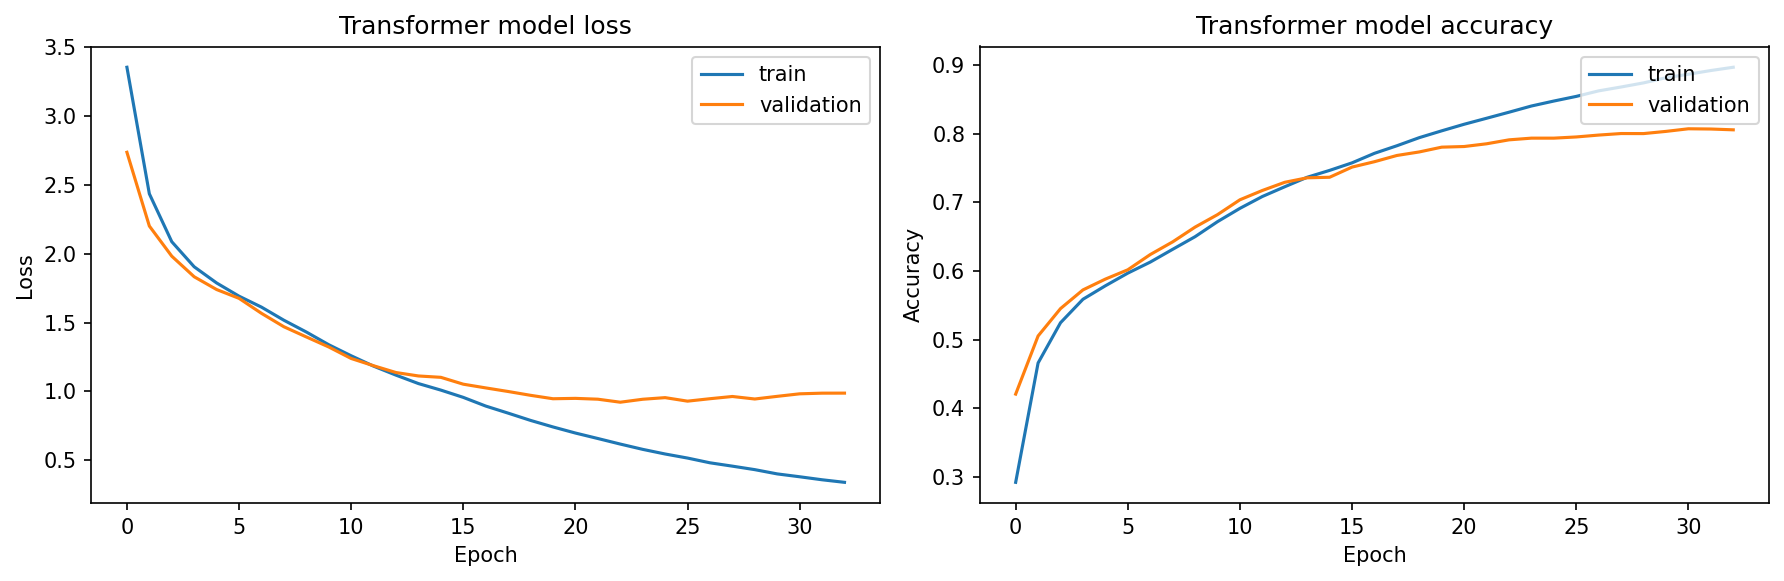
\includegraphics[width=\textwidth]{pic/training_history_mathwriting}
    \caption{\texttt{MathWriting-human} 上的训练曲线：验证损失于第 23 轮触底后走平，
    训练损失持续下降，呈现明显过拟合}
    \label{fig:training-history-mathwriting}
\end{figure}

两个数据集上的完整结果对比如表~\ref{tab:dataset-comparison} 所示。

\begin{table}[H]
    \centering
    \caption{印刷体与手写体数据集上的性能对比（相同架构与训练配方）}
    \begin{tabular}{lcc}
        \toprule
        \textbf{指标} & \texttt{im2latex-100k}（印刷体） & \texttt{MathWriting-human}（手写体） \\
        \midrule
        词表大小 & $504$ & $235$ \\
        训练轮数（早停） & $78$ & $33$ \\
        最优验证损失 & $0.4427$ & $0.9215$ \\
        最优验证掩蔽准确率 & $90.5\%$ & $\approx 79\%$ \\
        测试损失 & $0.4551$ & $2.1402$ \\
        测试掩蔽准确率 & $90.14\%$ & $56.63\%$ \\
        BLEU-4（贪婪解码） & $0.6767$ & $0.0833$ \\
        BLEU-4（束搜索，$k=4$） & $0.7012$ & $0.0786$ \\
        \bottomrule
    \end{tabular}
    \label{tab:dataset-comparison}
\end{table}

\subsubsection{性能差距的成因分析}
手写体上的性能大幅下降并非单一因素所致：以下前三点为模型与数据层面、可分别施治的成因，第四点则为评测指标对短序列的放大效应（属测量层面，而非模型本身缺陷），具体如下：
\begin{enumerate}[label={（\arabic*）}, leftmargin=2em, labelsep=0.5em, itemsep=0pt]
    \item {书写者分布偏移（最主要因素）}：验证集与训练集取自同一批样本的随机划分，
    二者共享书写者与书写风格，故验证准确率高达约 $79\%$；
    而测试划分来自独立的数据来源，测试准确率骤降至 $56.63\%$（测试损失 $2.14$ 对验证 $0.92$）。
    这一验证--测试鸿沟在印刷体实验中几乎不存在（$0.4427$ 对 $0.4551$），
    定量刻画了手写识别特有的跨书写者泛化难题；
    \item {样本量不足导致的过拟合}：印刷体的视觉模式高度标准化，$50{,}000$ 个样本已足够；
    手写体的同一符号在不同书写者笔下差异巨大，相同样本量下模型转而记忆训练样本的个体特征，
    训练曲线的提前分化即为直接证据。本实验为保证与印刷体严格可比而未使用
    \texttt{MathWriting-human} 的全部约 $230{,}000$ 个训练样本，也未引入任何数据增强；
    \item {几何失真}：手写采集图像的宽高比接近 $1{:}1.3$（如 $187\times141$），
    被强制缩放至 $50\times200$（宽高比 $4{:}1$）时产生严重的横向拉伸，
    笔画形态信息损失远大于本身即为宽幅排版的印刷体公式图像；
    \item {BLEU 对短参考序列的敏感性}：手写数据集的公式整体较短（不少参考序列不足 $10$ 个词元），
    BLEU-4 的高阶 $n$-gram 在短序列上极易失配，对相同的词元级错误率给出远低于长序列的分数，
    放大了两个数据集间生成指标的表观差距。
\end{enumerate}

此外，束搜索在手写体上未带来增益（$0.0786$ 对 $0.0833$）。
这与解码理论的预期一致：束搜索的收益建立在模型条件分布校准良好的前提上，
当模型本身欠拟合目标分布时，搜索更宽只会更彻底地利用一个不可靠的概率模型，
长度惩罚在大量短序列上的归一化也会进一步引入偏差。
该结果亦与表~\ref{tab:decoding} 的印刷体实验相呼应：束搜索的增益依赖于模型条件分布的校准质量，而非搜索算法本身；但二者序列长度分布差异较大，此处仅作定性参照。

定性考察（图~\ref{fig:predictions-mathwriting}）与上述分析吻合：
模型生成的序列几乎全部语法合法——分式、上下标乃至括号内的矩阵结构均能正确组织，
说明解码器习得的 LaTeX 语法先验迁移良好；笔迹清晰、结构简单的样本亦能被完整正确识别
（如图~\ref{fig:predictions-mathwriting} 左上样本所示的积分关系式 $\int \mathrm{d}V\,|\Psi|^{2}=N$ 被逐词元准确还原）。
但生成内容与图像的对应关系明显弱于印刷体，最典型的是“结构正确但符号识别有误”的输出——
例如图~\ref{fig:predictions-mathwriting} 右上样本正确还原了括号内的二行矩阵结构，
却把分子 $2r-1$ 误识为 $n+1$；表明主要瓶颈在于模型对手写笔迹的视觉特征提取与跨模态对齐，
而非语言建模能力。

\begin{figure}[H]
    \centering
    
\includegraphics[width=\textwidth]{pic/predictions_mathwriting}
    \caption{\texttt{MathWriting-human} 测试样本的预测结果与真实标签对照（左上为正确识别，右上为结构正确但符号识别有误，下方两例为错误识别）}
    \label{fig:predictions-mathwriting}
\end{figure}

\subsection{定性分析与误差分析}
本节针对印刷体（\texttt{im2latex-100k}）实验的生成结果展开定性与误差分析。
\subsubsection{生成质量的定性考察}
图~\ref{fig:predictions} 展示了测试集样本的预测结果与真实标签对照。
对测试集随机样本的人工考察表明，模型生成的 LaTeX 序列绝大多数语法完整、花括号正确配对，
能够直接通过 LaTeX 编译。模型对多种复杂结构均能正确建模，包括：
嵌套分式与根式（如 $\texttt{\textbackslash sqrt\{\textbackslash frac\{...\}\{...\}\}}$）、
多重上下标与张量指标链、求和与积分的上下限结构、
函数算符（\texttt{\textbackslash operatorname\{sin\}}、$\texttt{\textbackslash operatorname*\{lim\}}$）乃至
\texttt{\textbackslash begin\{array\}} 环境下的矩阵与行列式
（如图~\ref{fig:demo-samples}（b）所示的 $2\times2$ 分块行列式，其 \texttt{array} 主体结构被正确还原，仅末项的行列式定界符 $\lvert\cdot\rvert$ 被误生成为方括号）。

\begin{figure}[H]
    \centering
    
\includegraphics[width=\textwidth]{pic/predictions}
    \caption{测试集样本的预测结果（Predicted）与真实标签（Ground truth）对照}
    \label{fig:predictions}
\end{figure}

\begin{figure}[H]
    \centering
    \begin{subfigure}[b]{0.48\textwidth}
        \centering
        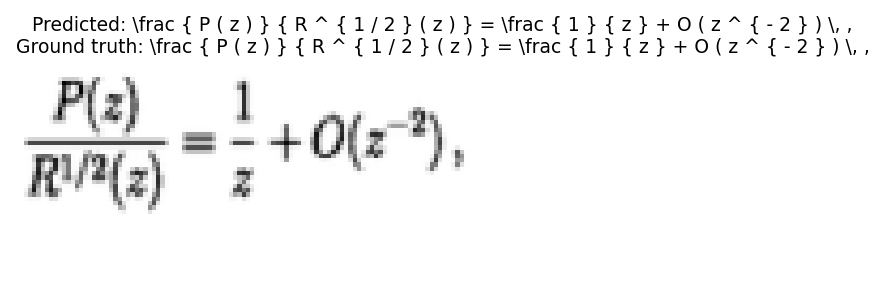
\includegraphics[width=\linewidth]{pic/demo_simple_sample}
        \caption{含渐近 $O$ 记号的分式表达式}
        \label{fig:demo-simple}
    \end{subfigure}
    \hfill
    \begin{subfigure}[b]{0.48\textwidth}
        \centering
        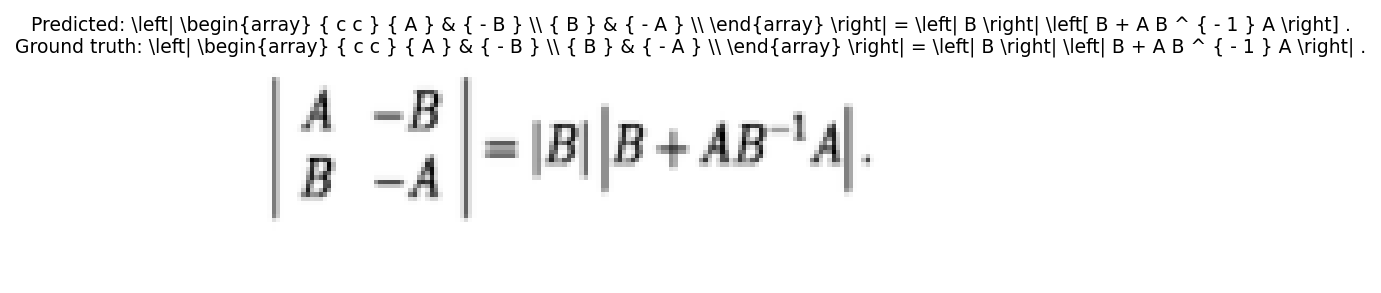
\includegraphics[width=\linewidth]{pic/demo_array_sample}
        \caption{含 \texttt{array} 环境的分块行列式}
        \label{fig:demo-array}
    \end{subfigure}
    \caption{随机测试样本的生成结果示例}
    \label{fig:demo-samples}
\end{figure}

\subsubsection{典型错误模式}
对生成失败的样本进行归类，主要错误模式及其成因如下：
\begin{enumerate}[label={（\arabic*）}, leftmargin=2em, labelsep=0.5em, itemsep=0pt]
    \item {相似符号混淆}：低分辨率输入（$50\times200$）下视觉上相近的符号易被混淆，
    如上下标位置的数字与字母、$\texttt{\textbackslash partial}$ 与 $\partial$ 形近符号等。
    此类错误为单词元替换，对 BLEU 的高阶 $n$-gram 影响有限但直接影响语义正确性；
    \item {长序列后段退化}：在较长表达式的生成后段偶见词元序列退化
    （如下标中字母被逐个拆散为无意义组合），
    反映了自回归解码误差累积与低分辨率下细节信息不足的叠加效应；
    \item {括号失配残留}：极少数样本存在多余或缺失的右花括号或
    \texttt{\textbackslash left}/\texttt{\textbackslash right} 定界符失配，
    导致编译失败。该类错误源于模型缺乏对括号配对的显式约束，
    完全依赖数据驱动的隐式学习；
    \item {词表外词元不可生成}：词表基于 $50{,}000$ 个训练样本构建（$504$ 个词元），
    测试集中出现的词表外（OOV）词元被映射为 \texttt{[UNK]}，而 \texttt{[UNK]} 在输出层被先验偏置禁止生成，
    故含罕见命令的表达式必然无法完整复原。
    评估时此类位置已通过掩蔽机制从损失统计中排除，但其对 BLEU 的影响真实存在。
\end{enumerate}

\subsection{局限性与展望}
\label{subsec:limitations}
本文工作的主要局限与相应的改进方向如下：
\begin{enumerate}[label={（\arabic*）}, leftmargin=2em, labelsep=0.5em, itemsep=0pt]
    \item {输入分辨率}：$50\times200$ 的输入尺寸对长公式压缩严重，
    是相似符号混淆与细节丢失的首要原因。提高输入分辨率（并相应增大图像块数量）
    是性能提升空间最明确的方向，其代价是自注意力计算量随图像块数二次增长；
    \item {模型容量}：$7.73$M 的参数规模远小于该任务的专用模型，
    在训练数据充足的前提下，加深加宽模型有望进一步缩小与专用方法的差距；
    \item {解码约束}：当前解码过程无语法约束，括号失配等结构性错误只能依靠数据隐式纠正。
    引入语法感知的约束解码或树结构解码器\supercite{zhuTAMERTreeawareTransformer2024}
    是改善结构正确性的可行途径；
    \item {手写场景的针对性改进}：第~\ref{subsec:handwriting} 节的对比实验定量揭示了
    直接迁移印刷体配方的三个瓶颈，对应的改进方向均有明确依据：
    针对跨书写者泛化与过拟合，应使用 \texttt{MathWriting-human} 的全部约 $230{,}000$
    个训练样本并配合数据增强（随机仿射变换、弹性形变）；
    针对几何失真，应采用保持宽高比的缩放加填充策略替代直接拉伸；
    在此基础上再叠加更高输入分辨率，预期可显著缩小手写与印刷体之间的性能差距。
\end{enumerate}

综上，本文构建的 ViT 编码器--Transformer 解码器模型在印刷体数据集 \texttt{im2latex-100k} 上
取得了 $90.14\%$ 的词元级准确率与 $0.7012$ 的 BLEU-4 分数（束搜索解码），
以轻量的模型规模与低分辨率输入验证了纯 Transformer 架构在数学表达式识别与 LaTeX
转换任务上的有效性；训练稳定性分析为大批量预热调度下梯度裁剪的必要性提供了直接的实验证据；
手写体对比实验则在严格控制变量的前提下，将手写场景的难度定量分解为
书写者分布偏移、样本量不足与几何失真三个可分别施治的因素，为后续改进指明了路径。

\end{sloppypar}

\newpage
\addcontentsline{toc}{section}{参考文献}
\printbibliography[title={参考文献}]
\nocite{*}


% \begin{sloppypar}
%   \newpage\appendix
\renewcommand{\thesubsection}{\Alph{subsection}} % 为附录子章节添加编号 A, B, C, ...
\addcontentsline{toc}{section}{附\qquad 录}
\section*{\heiti\zihao{-2}附\qquad 录}
本研究的核心代码基于 PyTorch 实现，组织为 \texttt{vit\_latex} 程序包，按职责划分为数据处理（分词器与图像预处理）、模型组件（ViT 编码器、Transformer 解码器、生成模型）、训练（损失指标、学习率调度、训练循环）与评估四个子包，构建了从数学表达式图像到 LaTeX 序列的端到端转换流程。以下列出各核心模块的完整实现。
\subsection{代码一：超参数配置}
\lstinputlisting[label={lst:lst-config}]{../Code/vit_latex/config.py}
\subsection{代码二：LaTeX 分词器}
\lstinputlisting[label={lst:lst-tokenizer}]{../Code/vit_latex/data/tokenizer.py}
\subsection{代码三：图像预处理与数据加载}
\lstinputlisting[label={lst:lst-preprocessing}]{../Code/vit_latex/data/preprocessing.py}
\subsection{代码四：ViT 编码器}
\lstinputlisting[label={lst:lst-encoder}]{../Code/vit_latex/models/encoder.py}
\subsection{代码五：Transformer 解码器组件}
\lstinputlisting[label={lst:lst-decoder}]{../Code/vit_latex/models/decoder.py}
\subsection{代码六：生成模型与解码策略}
\lstinputlisting[label={lst:lst-captioner}]{../Code/vit_latex/models/captioner.py}
\subsection{代码七：损失函数与评价指标}
\lstinputlisting[label={lst:lst-metrics}]{../Code/vit_latex/training/metrics.py}
\subsection{代码八：优化器与学习率调度}
\lstinputlisting[label={lst:lst-scheduler}]{../Code/vit_latex/training/scheduler.py}
\subsection{代码九：模型训练}
\lstinputlisting[label={lst:lst-trainer}]{../Code/vit_latex/training/trainer.py}
\subsection{代码十：性能评估}
\lstinputlisting[label={lst:lst-evaluator}]{../Code/vit_latex/evaluation/evaluator.py}
\subsection{代码十一：主程序入口}
\lstinputlisting[label={lst:lst-main}]{../Code/main.py}

% \end{sloppypar}

\end{document}
